% !TEX root = ./final_report.tex
\section{Results \label{ref:results}}

\subsection{High Observation Noise in Lateral Axis: Point Target}

	In this model we make the assumption that the sensor available to the agent is capable of precisely measuring in the longitudinal direction, along the displacement vector between the particle and the agent position.  However, the measurement is quite noisy in the lateral direction.  The results are shown graphically in Figure \ref{fig:bad_heading}.  At the first decision point, the signal is very noisy in the direction lateral to the particles.  The algorithm determines that by measuring at different angles it can improve localization of the hostile vehicle. The agent continues to move around the target until there is no useful reduction of state uncertainty by moving or waiting available within the next $D$ time steps.  Thus the agent chooses to shoot, and successfully hits the target.
	
	% !TEX root = ./final_report.tex

\begin{figure}
        \centering
        \begin{subfigure}[b]{0.3\textwidth}
                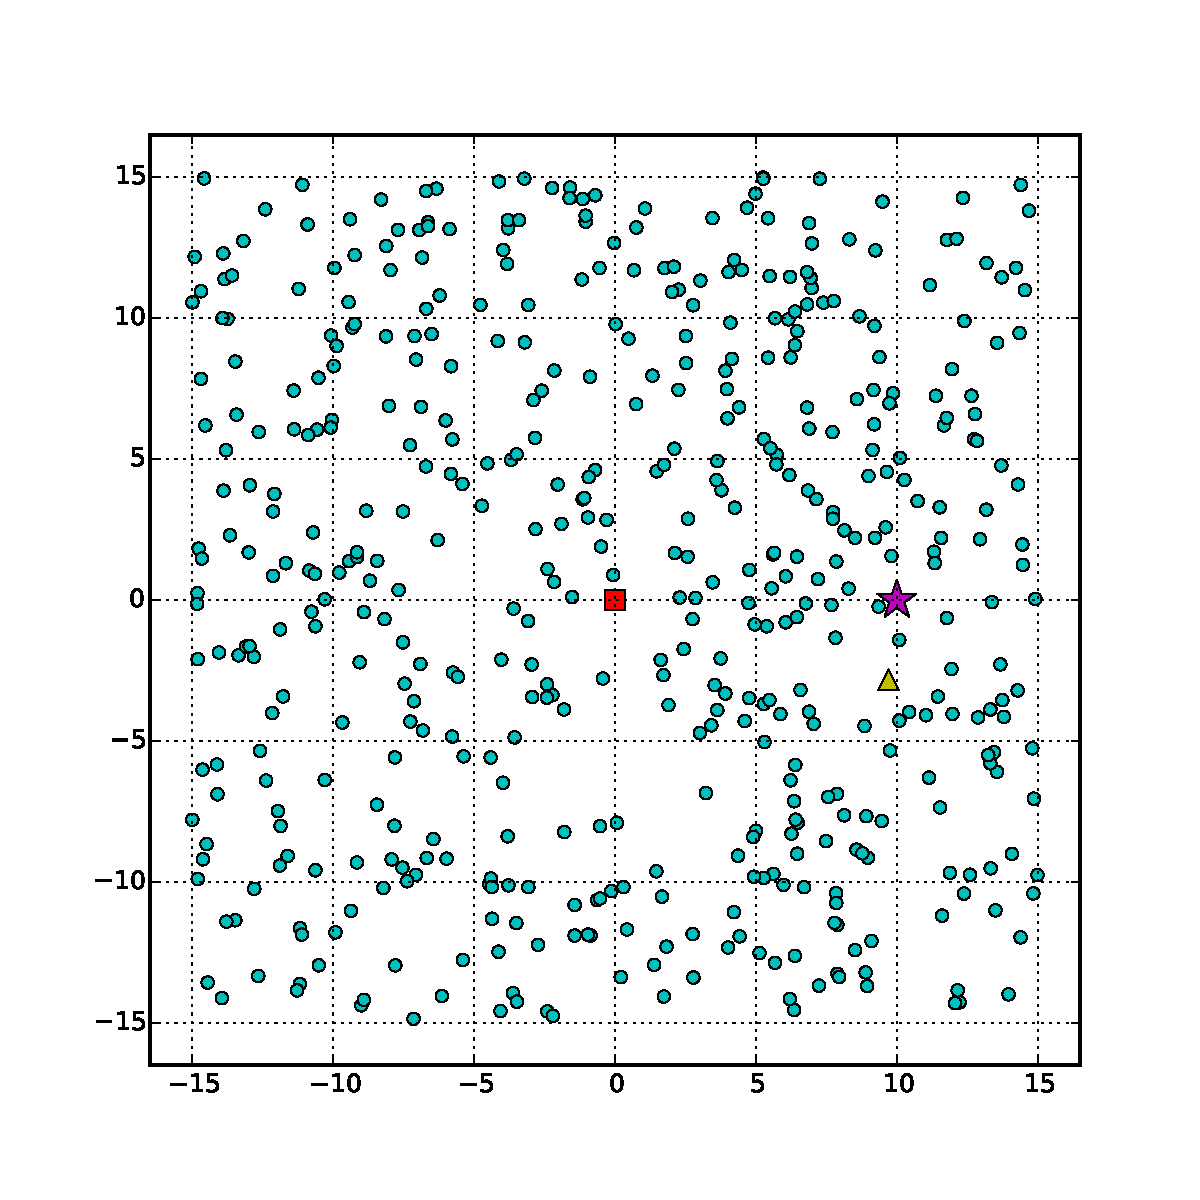
\includegraphics[width=\textwidth]{bad_heading_initial}
                \caption{Initial belief state}
                \label{fig:bad_heading_init}
        \end{subfigure}%
        ~ %add desired spacing between images, e. g. ~, \quad, \qquad, \hfill etc.
          %(or a blank line to force the subfigure onto a new line)
        \begin{subfigure}[b]{0.3\textwidth}
                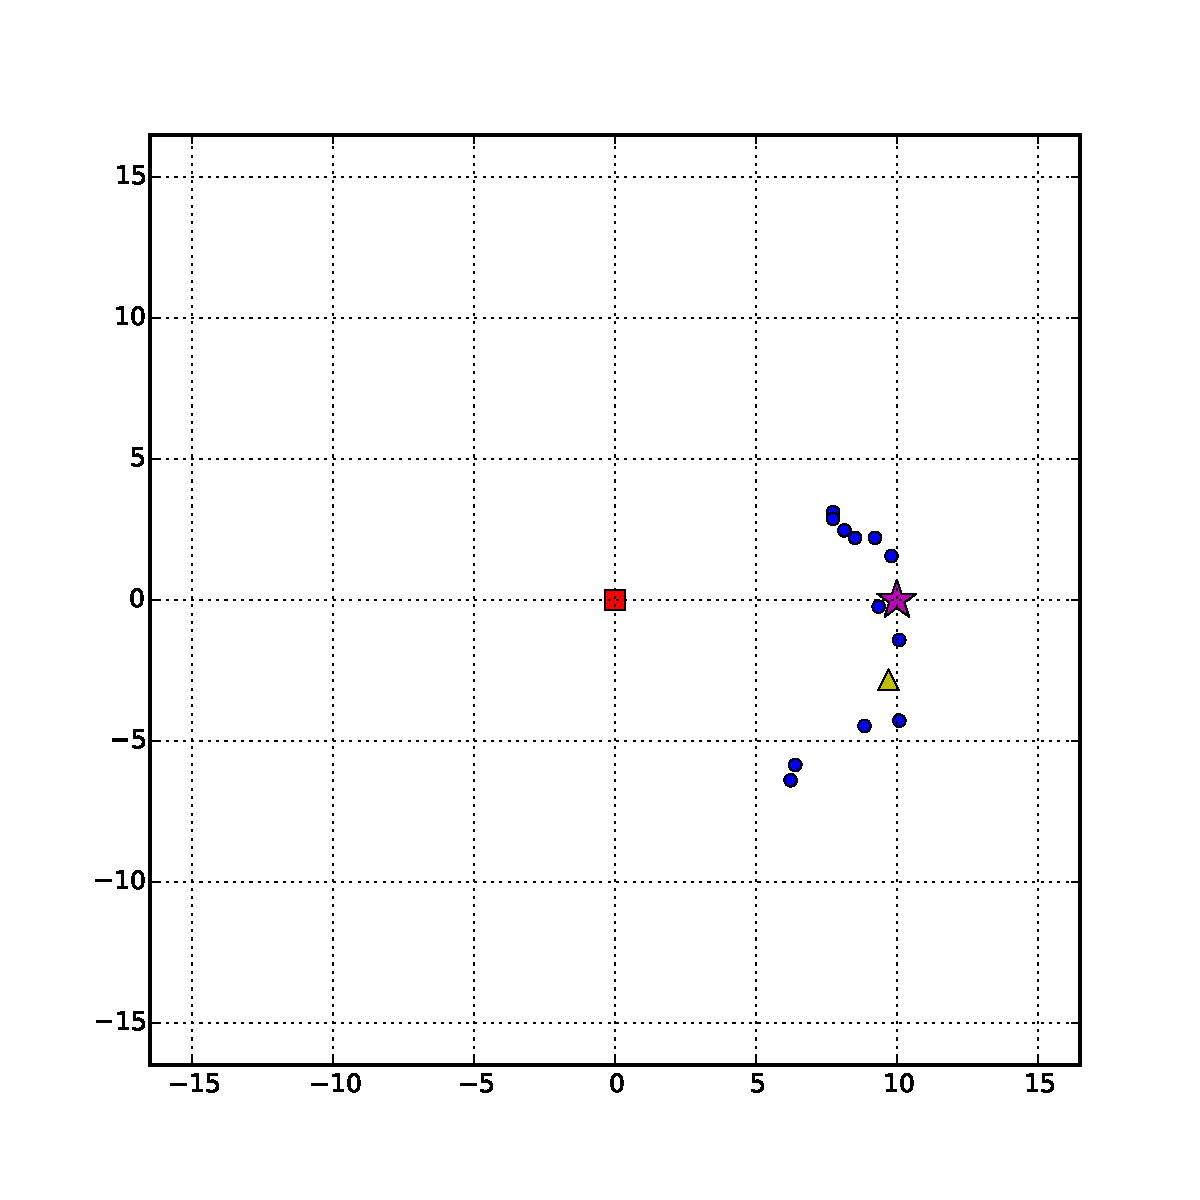
\includegraphics[width=\textwidth]{bad_heading_first_obs}
                \caption{t=0, first observation}
                \label{fig:bad_heading_t_0}
        \end{subfigure}
        ~ %add desired spacing between images, e. g. ~, \quad, \qquad, \hfill etc.
          %(or a blank line to force the subfigure onto a new line)
        \begin{subfigure}[b]{0.3\textwidth}
                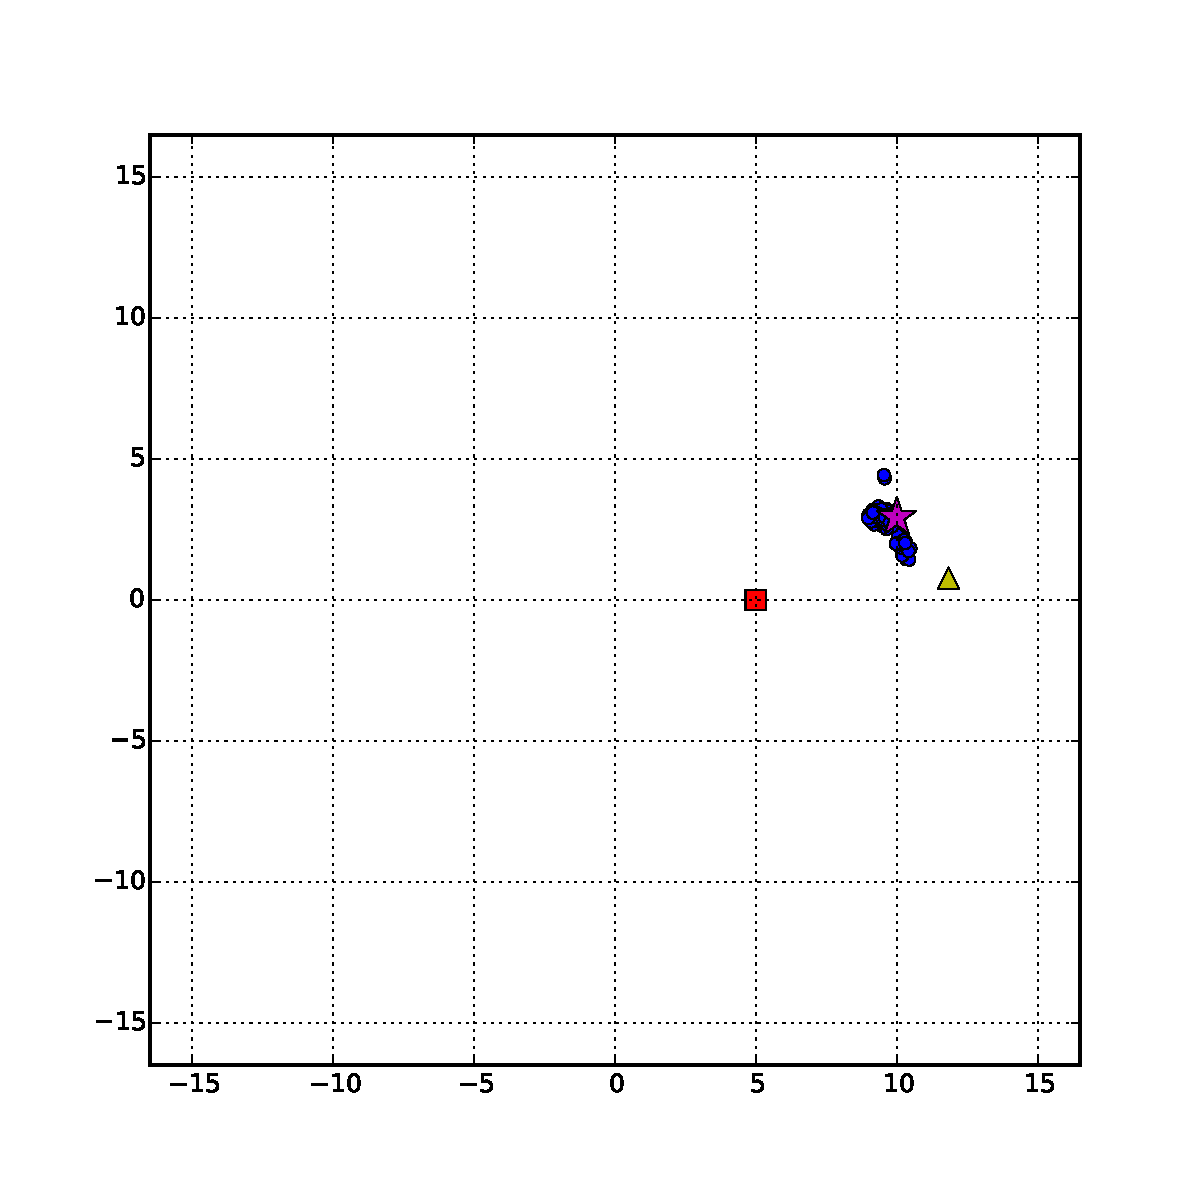
\includegraphics[width=\textwidth]{bad_heading_t_2}
                \caption{t=2}
                \label{fig:bad_heading_t_2}
        \end{subfigure}
        \begin{subfigure}[b]{0.3\textwidth}
                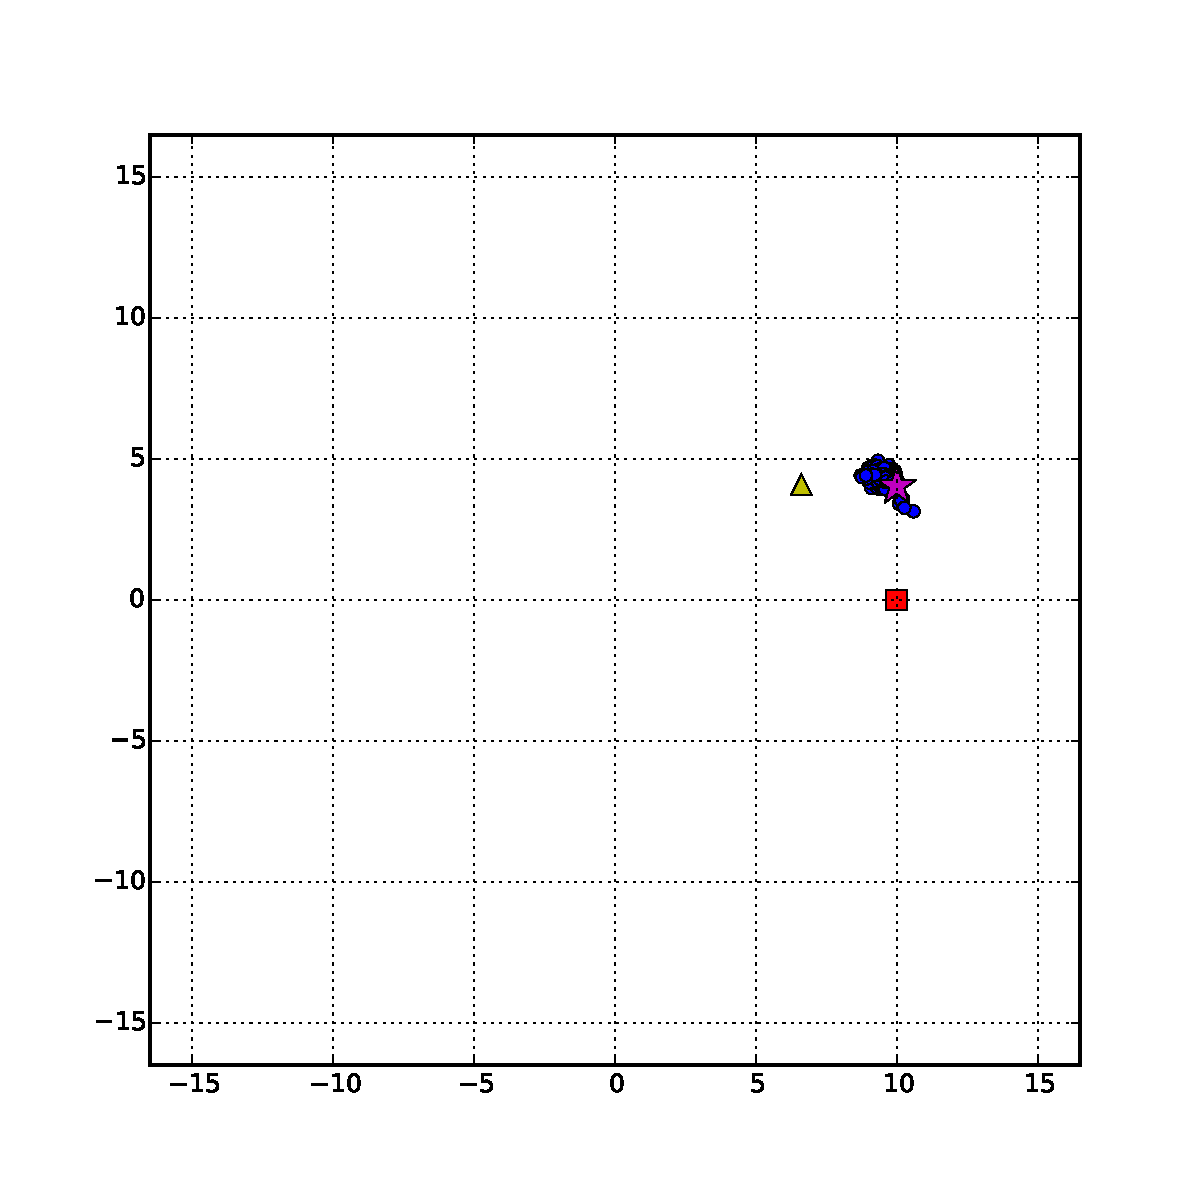
\includegraphics[width=\textwidth]{bad_heading_t_3}
                \caption{t=3}
                \label{fig:bad_heading_t_3}
        \end{subfigure}
        \begin{subfigure}[b]{0.3\textwidth}
                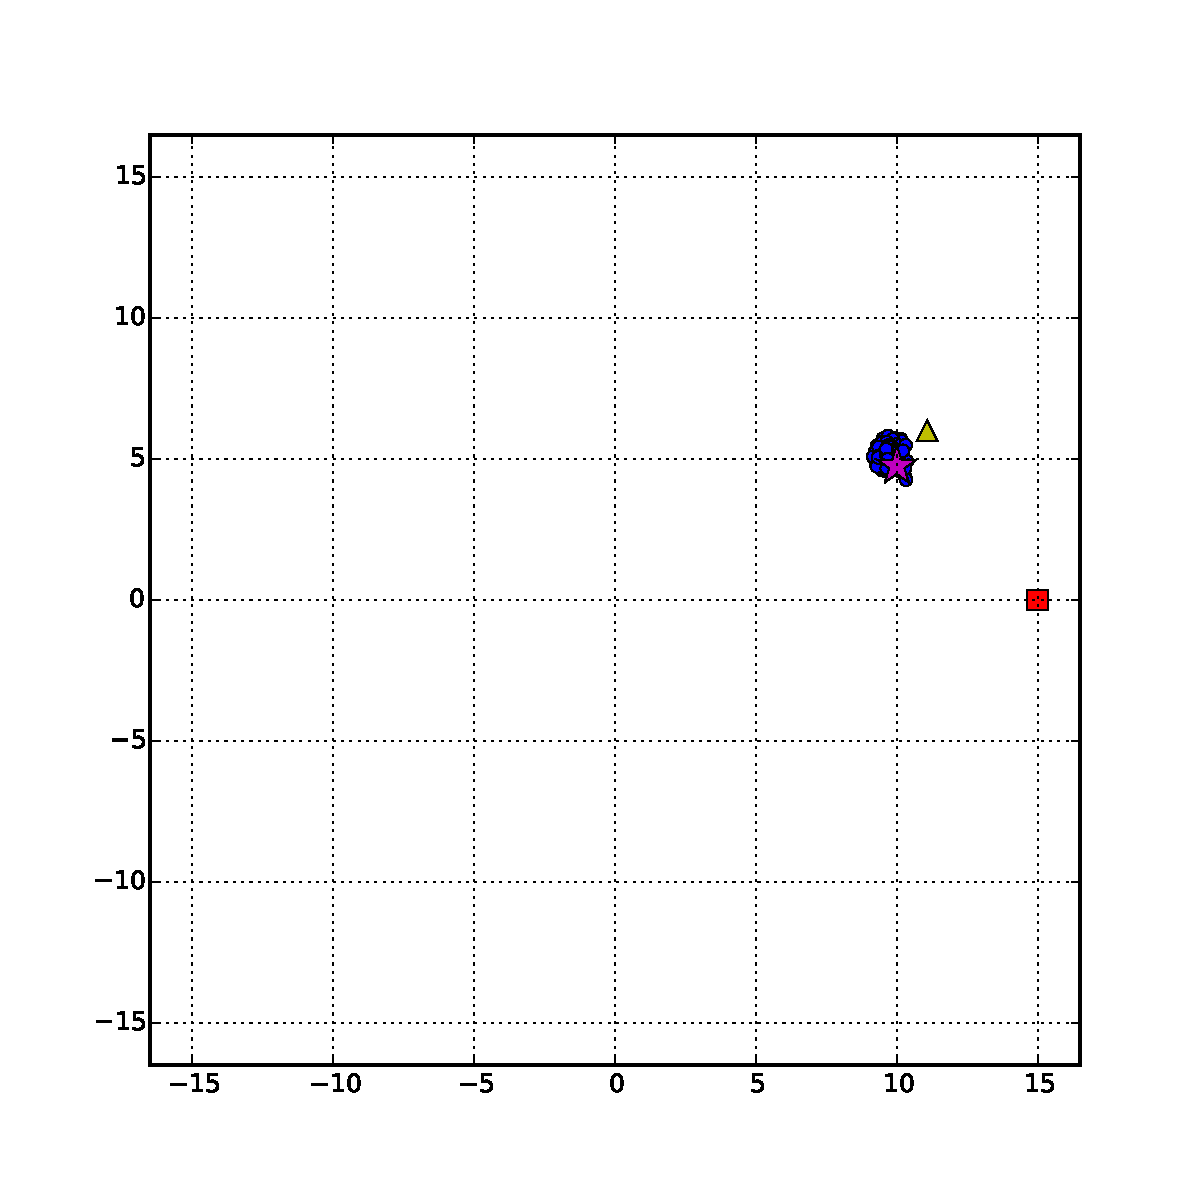
\includegraphics[width=\textwidth]{bad_heading_t_4}
                \caption{t=4}
                \label{fig:bad_heading_t_4}
        \end{subfigure}
        \begin{subfigure}[b]{0.3\textwidth}
                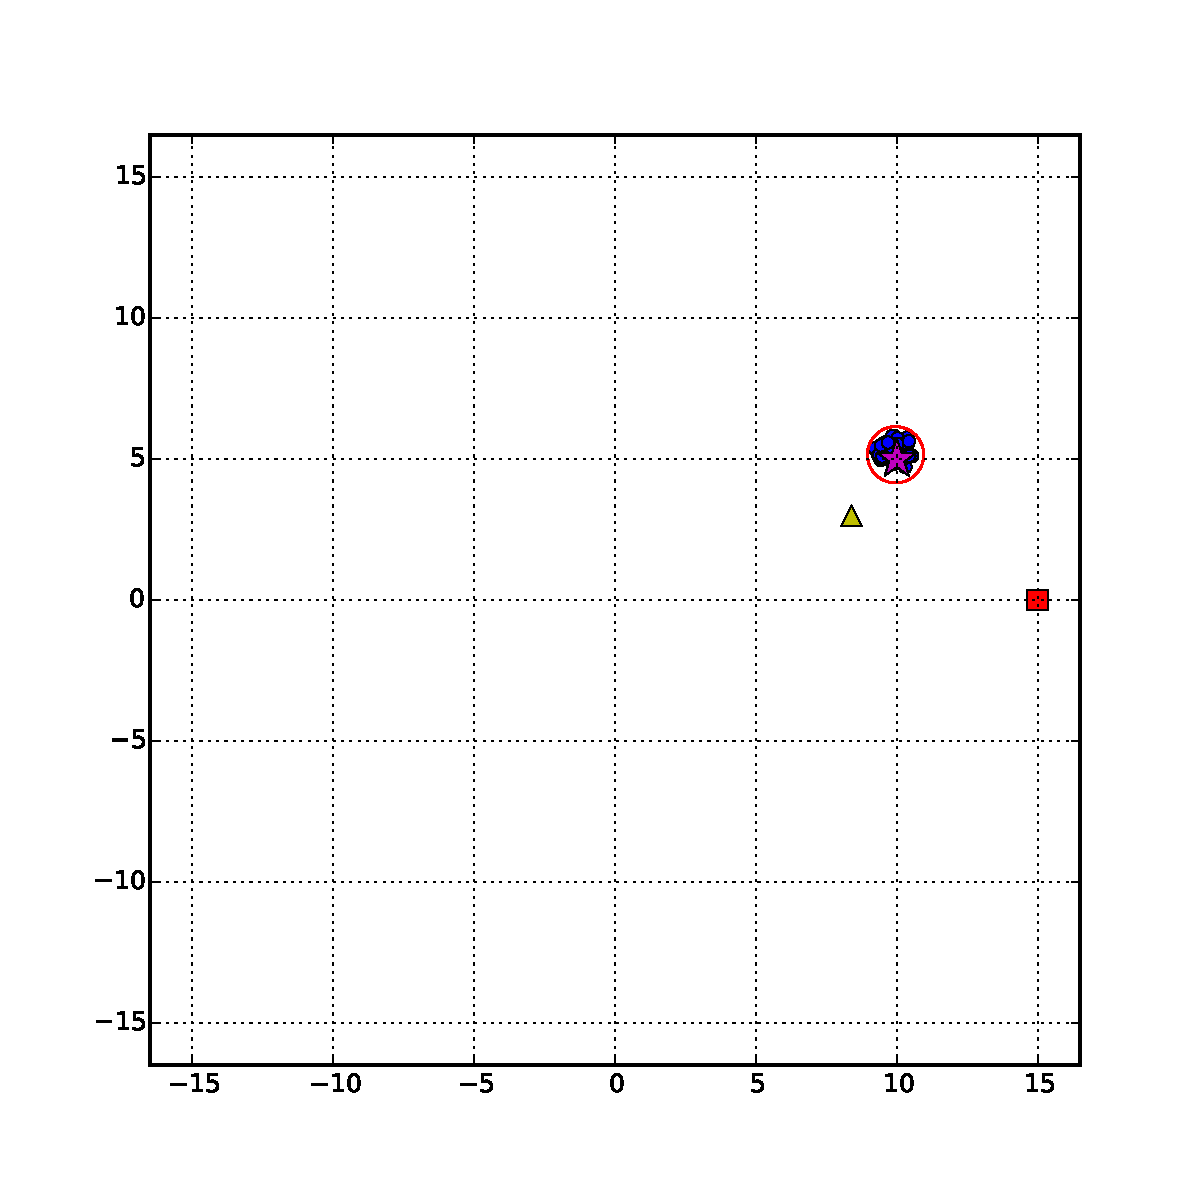
\includegraphics[width=\textwidth]{bad_heading_t_5}
                \caption{t=5, agent engages target}
                \label{fig:bad_heading_t_5}
        \end{subfigure}
        \caption{Progression of MC-RTBSS algorithm for the case where there is high lateral variance in the observation measurement, and the shooting mechanism is a point target. The agent state is the red square, the current observation is the yellow triangle, the true target position is the magenta star, the belief state particles are the blue circles, and the shooting mechanism is the red circle.}\label{fig:bad_heading}
\end{figure}
	
\subsection{High Observation Noise in Lateral Axis: Angle Target}
	We make the assumption in this model that the sensor available to the agent is capable of precisely measuring in the longitudinal direction, along the displacement vector between the particle and the agent position.  However, the measurement is quite noisy in the lateral direction.  The results are shown graphically in Figure \ref{fig:beam_bad_heading}.  At the first decision point, the signal is very noisy in the direction lateral to the particles.  The algorithm determines that by measuring at different angles it can improve localization of the hostile vehicle.  Additionally by moving away from the vehicle the beam width at target intersection is much larger.  The moves mostly down at first, as this is the most effective way to change measurement angle, which will most rapidly reduce the uncertainty of the belief state.  Once the agent reaches the game boundary in the vertical axis, it resumes moving away to the left.  Once it is as far from the target as possible, the algorithm returns that there is no useful reduction of state uncertainty or increase of beam width at target intersection within the next $D$ time steps.  Thus the agent chooses to shoot, and successfully hits the target.
	
	% !TEX root = ./final_report.tex

\begin{figure}
        \centering
        \begin{subfigure}[b]{0.3\textwidth}
                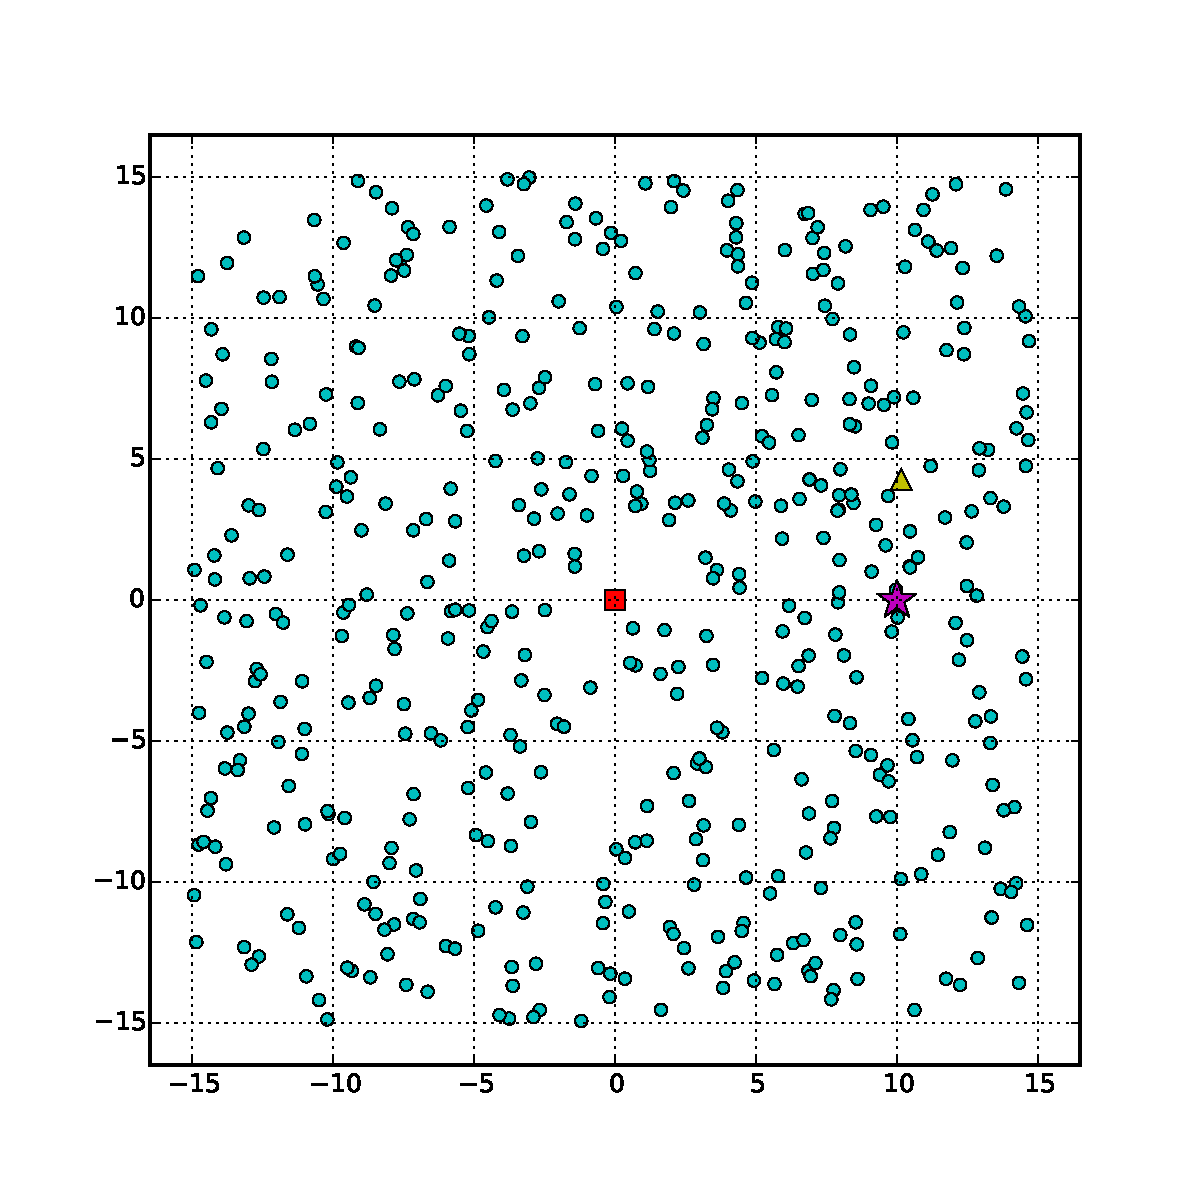
\includegraphics[width=\textwidth]{beam_bad_heading_initial}
                \caption{Initial belief state}
                \label{fig:beam_bad_heading_init}
        \end{subfigure}%
        ~ %add desired spacing between images, e. g. ~, \quad, \qquad, \hfill etc.
          %(or a blank line to force the subfigure onto a new line)
        \begin{subfigure}[b]{0.3\textwidth}
                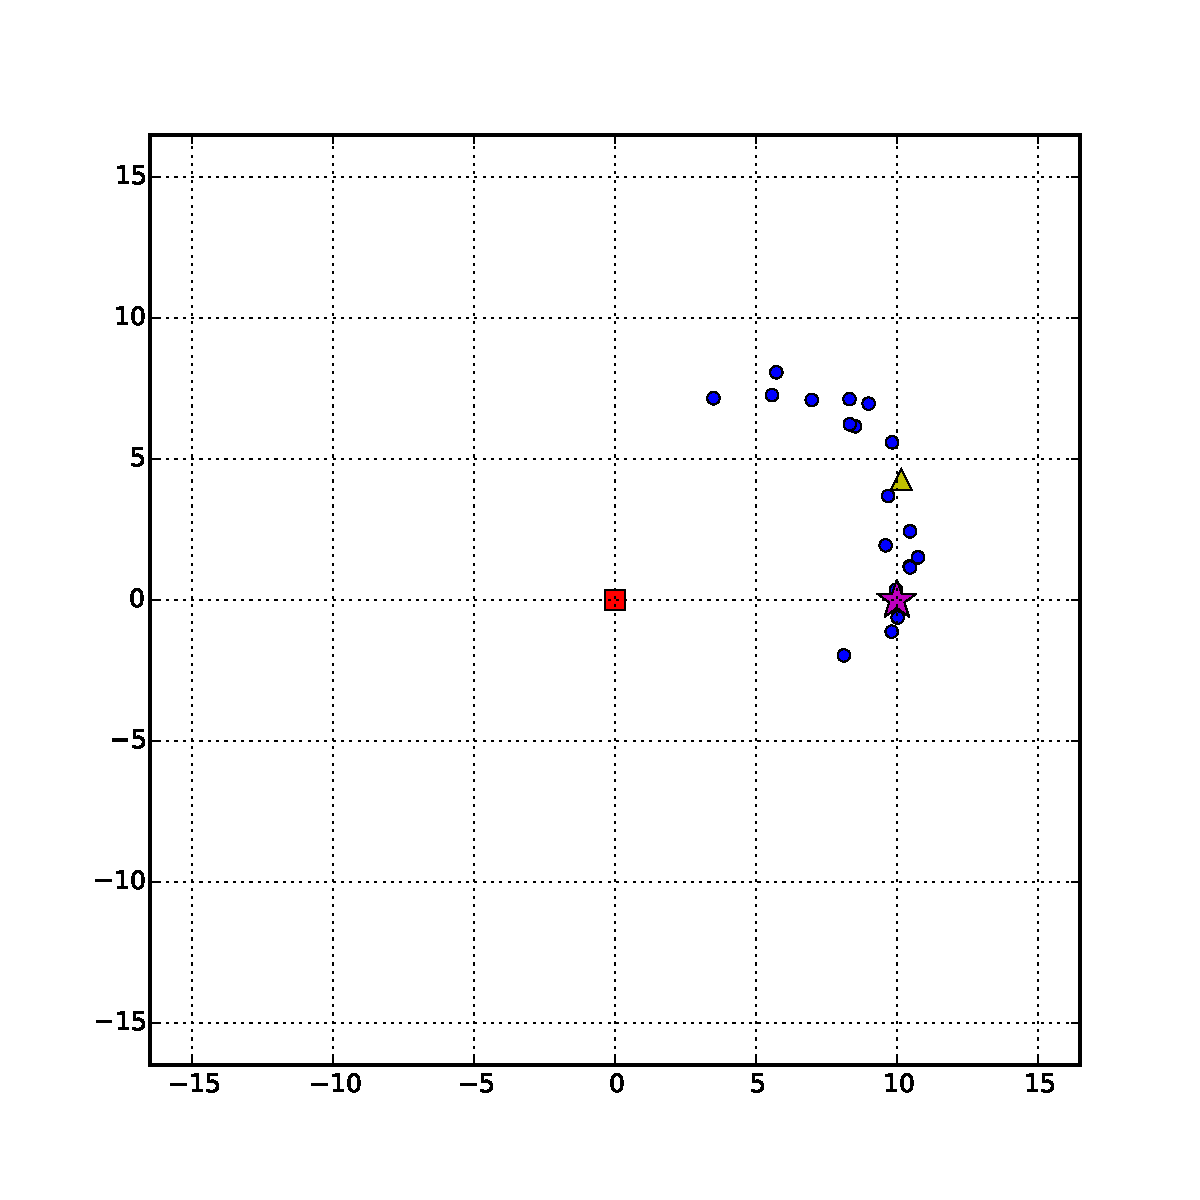
\includegraphics[width=\textwidth]{beam_bad_heading_first_obs}
                \caption{A t=0, first observation}
                \label{fig:beam_bad_heading_t_0}
        \end{subfigure}
        ~ %add desired spacing between images, e. g. ~, \quad, \qquad, \hfill etc.
          %(or a blank line to force the subfigure onto a new line)
        \begin{subfigure}[b]{0.3\textwidth}
                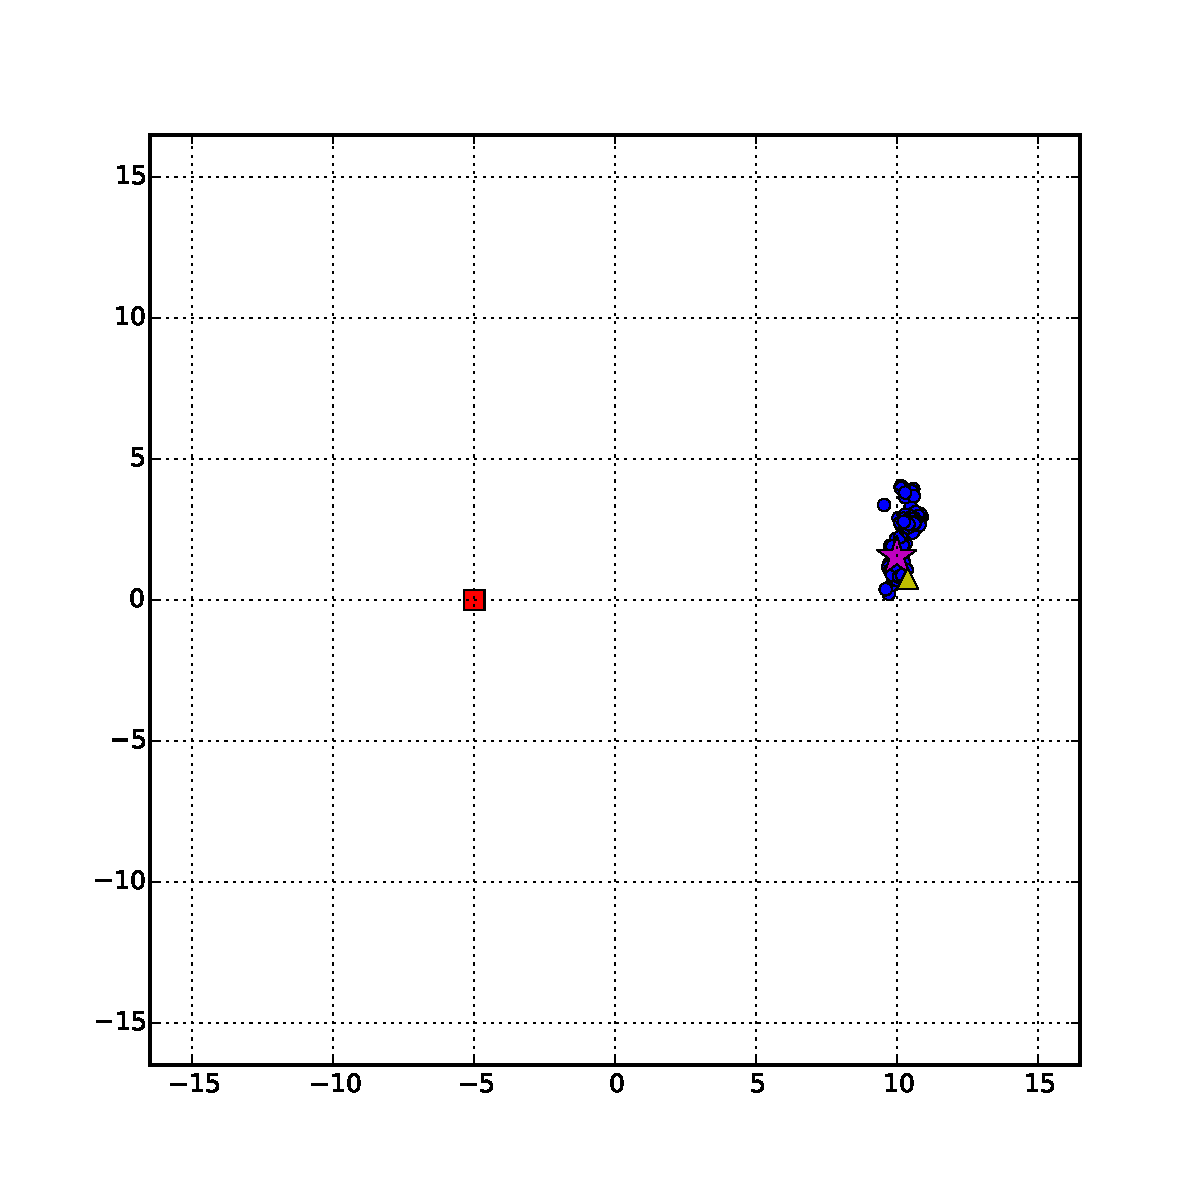
\includegraphics[width=\textwidth]{beam_bad_heading_t_1}
                \caption{t=1}
                \label{fig:beam_bad_heading_t_1}
        \end{subfigure}
        \begin{subfigure}[b]{0.3\textwidth}
                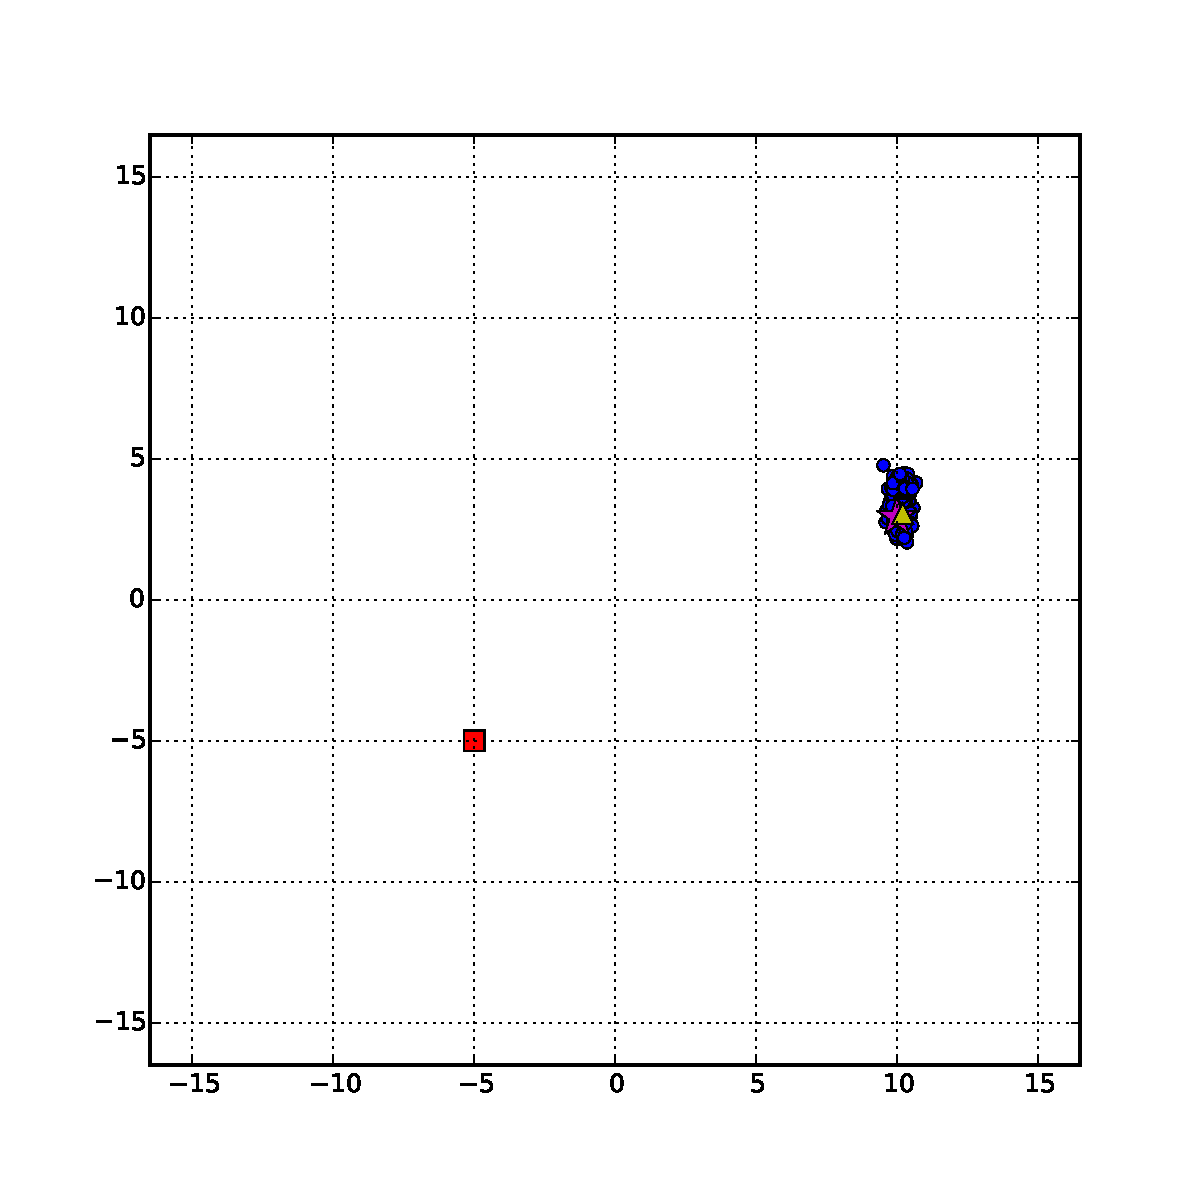
\includegraphics[width=\textwidth]{beam_bad_heading_t_2}
                \caption{t=2}
                \label{fig:beam_bad_heading_t_2}
        \end{subfigure}
        \begin{subfigure}[b]{0.3\textwidth}
                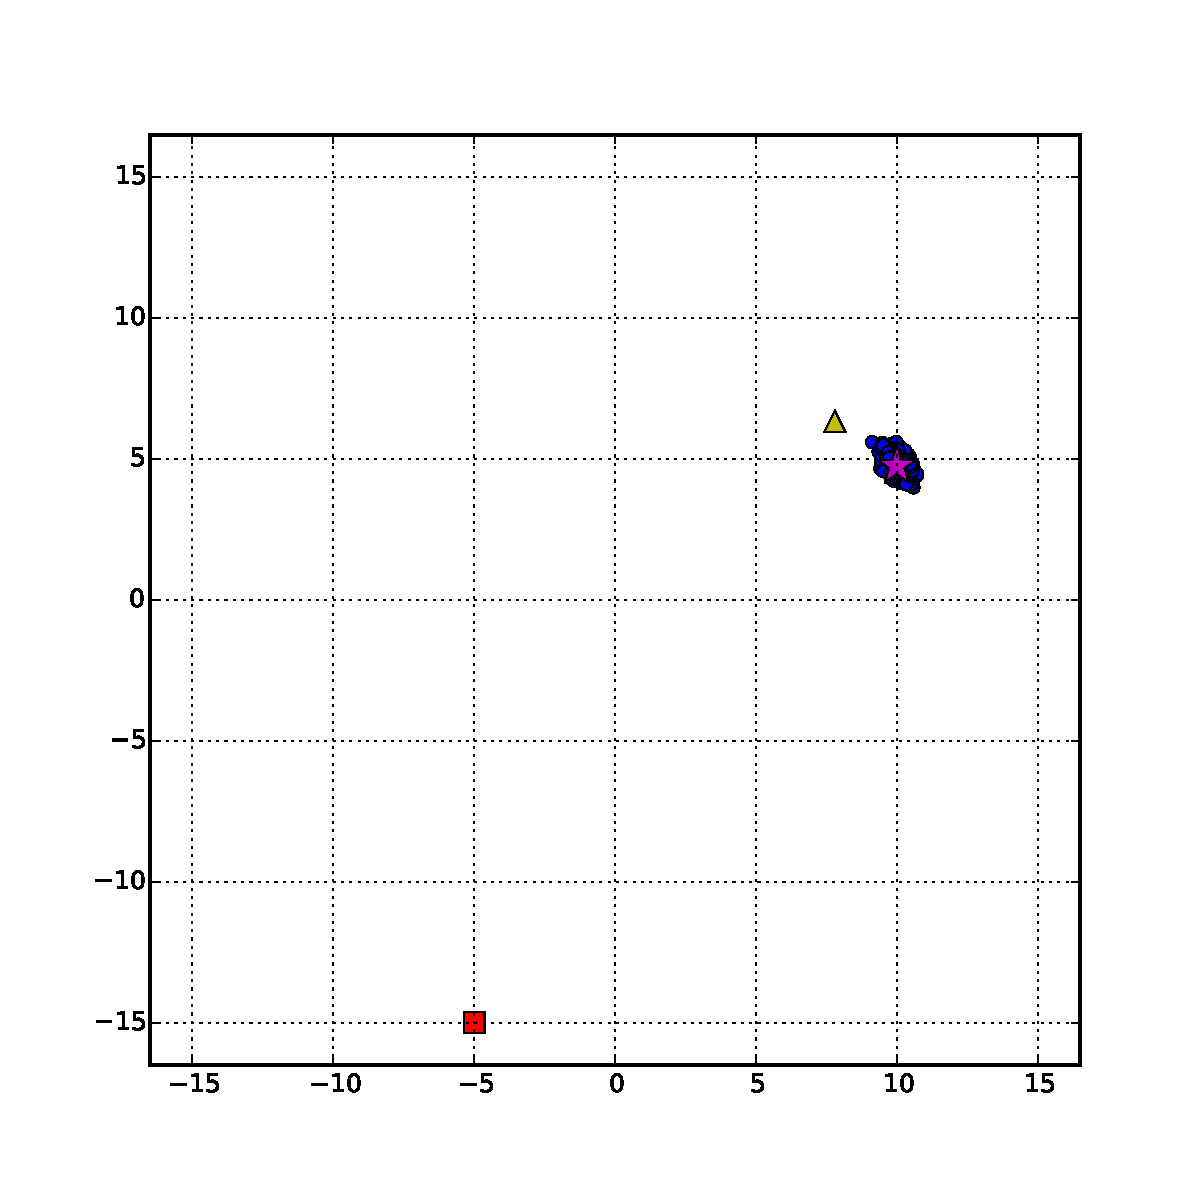
\includegraphics[width=\textwidth]{beam_bad_heading_t_4}
                \caption{t=4}
                \label{fig:beam_bad_heading_t_4}
        \end{subfigure}
        \begin{subfigure}[b]{0.3\textwidth}
                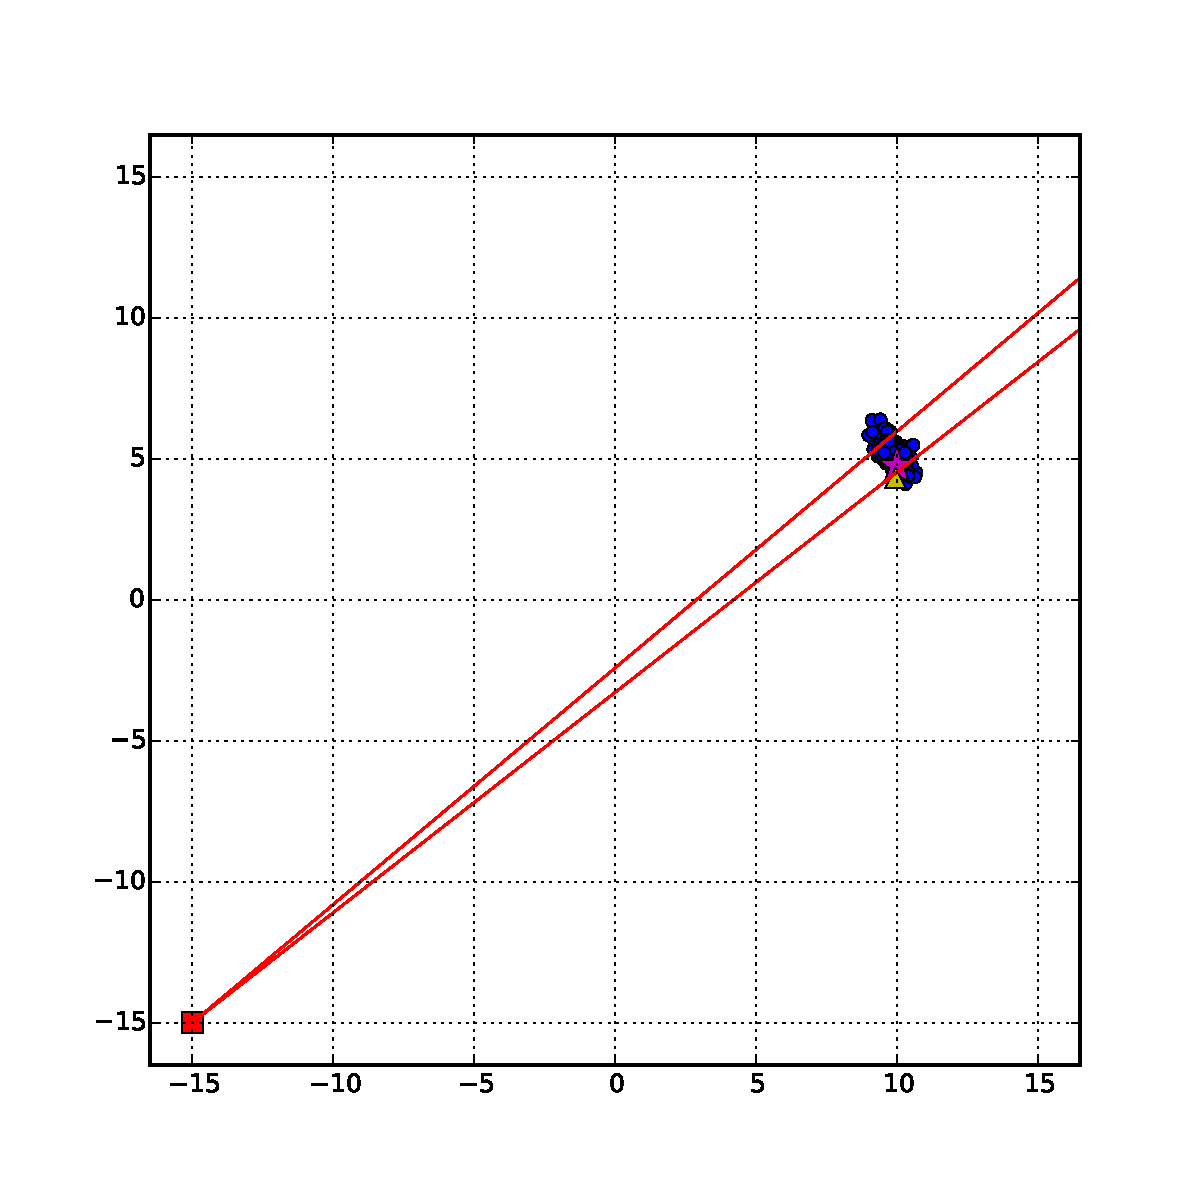
\includegraphics[width=\textwidth]{beam_bad_heading_t_6}
                \caption{t=6, agent engages target}
                \label{fig:beam_bad_heading_t_6}
        \end{subfigure}
        \caption{Progression of MC-RTBSS algorithm for the case where there is high lateral variance in the observation measurement, and the shooting mechanism is an angle target. The agent state is the red square, the current observation is the yellow triangle, the true target position is the magenta star, the belief state particles are the blue circles, and the shooting mechanism is the red beam.}\label{fig:beam_bad_heading}
\end{figure}

\subsection{High Transition Velocity Noise: Angle Target}
	In this model we assumed that the hostile vehicle is not able to control the magnitude of its velocity very precisely.  Thus, as particles are transitioned or projected forward, the position uncertainty is much larger in the direction of travel.  The results are shown in the plots of Figure \ref{fig:vel_noise}.  In this case, the agent begins by moving to the right.  This is because the reward function will most quickly increase by reducing the angle between the displacement vector and the major principle axis of the velocity noise.  Once the agent is directly down from the target vehicle, it moves further downward.  The algorithm is able to determine that the total game reward can be further increased by using another time step to reduce the angular spread of the target, and thus increase the proportion of belief states covered by the beam.  After that final adjustment, the algorithm does not detect any improvement in chance to hit the target that will be worth the additional time cost.  In this example the agent shoots and hits the target.
	
	% !TEX root = ./final_report.tex

\begin{figure}
	    \centering
	    \begin{subfigure}[b]{0.3\textwidth}
	            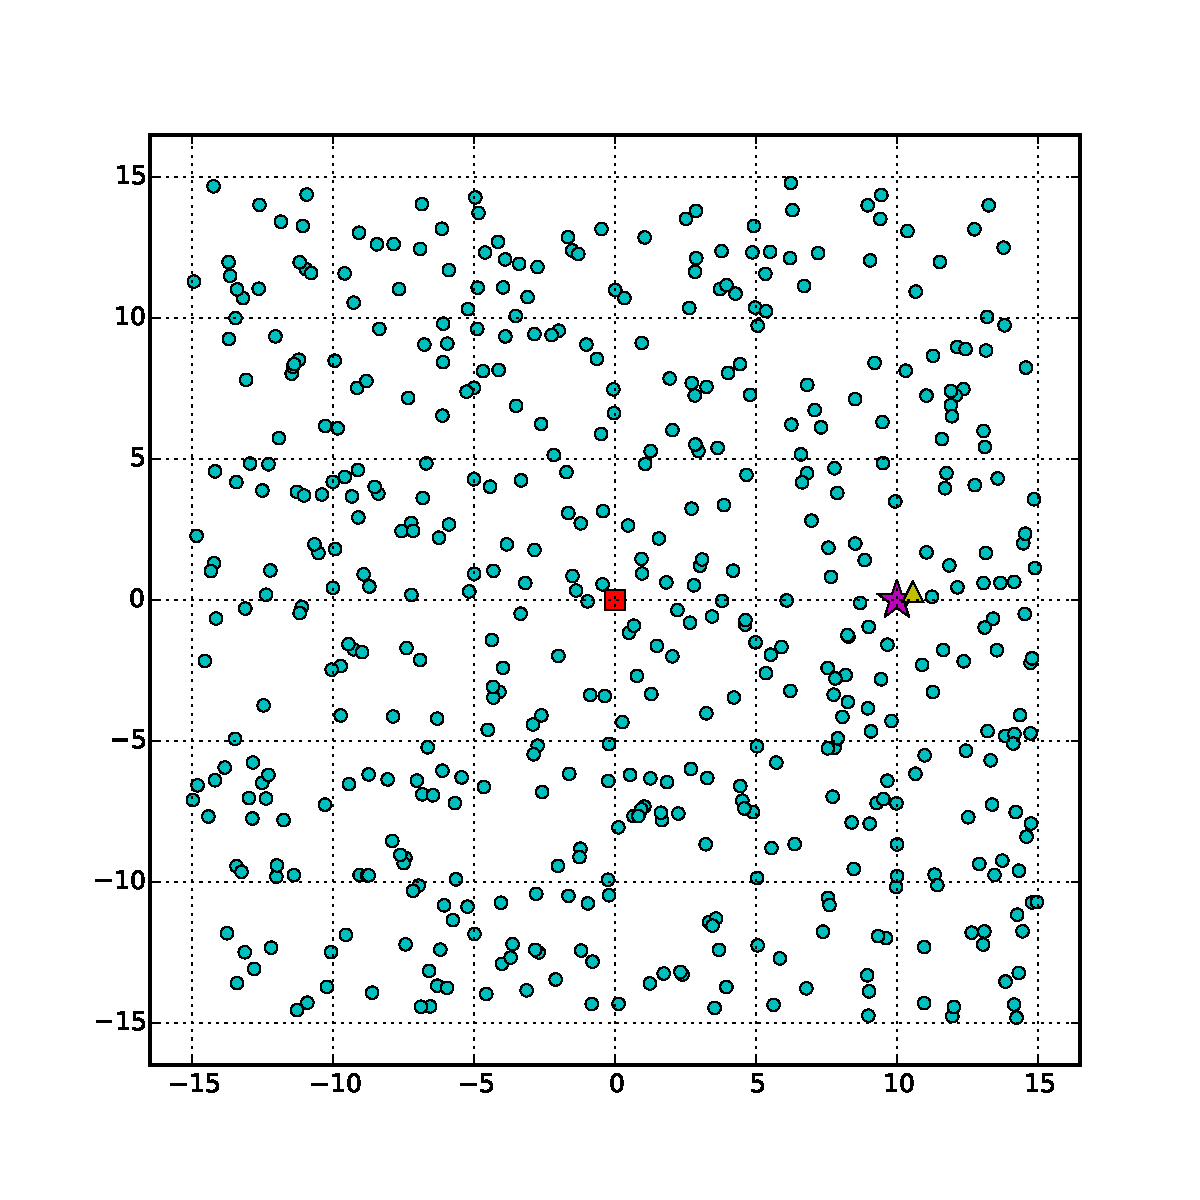
\includegraphics[width=\textwidth]{high_vel_noise_initial}
	            \caption{Initial belief state}
	            \label{fig:high_vel_noise_init}
	    \end{subfigure}%
	    ~ %add desired spacing between images, e. g. ~, \quad, \qquad, \hfill etc.
	      %(or a blank line to force the subfigure onto a new line)
	    \begin{subfigure}[b]{0.3\textwidth}
	            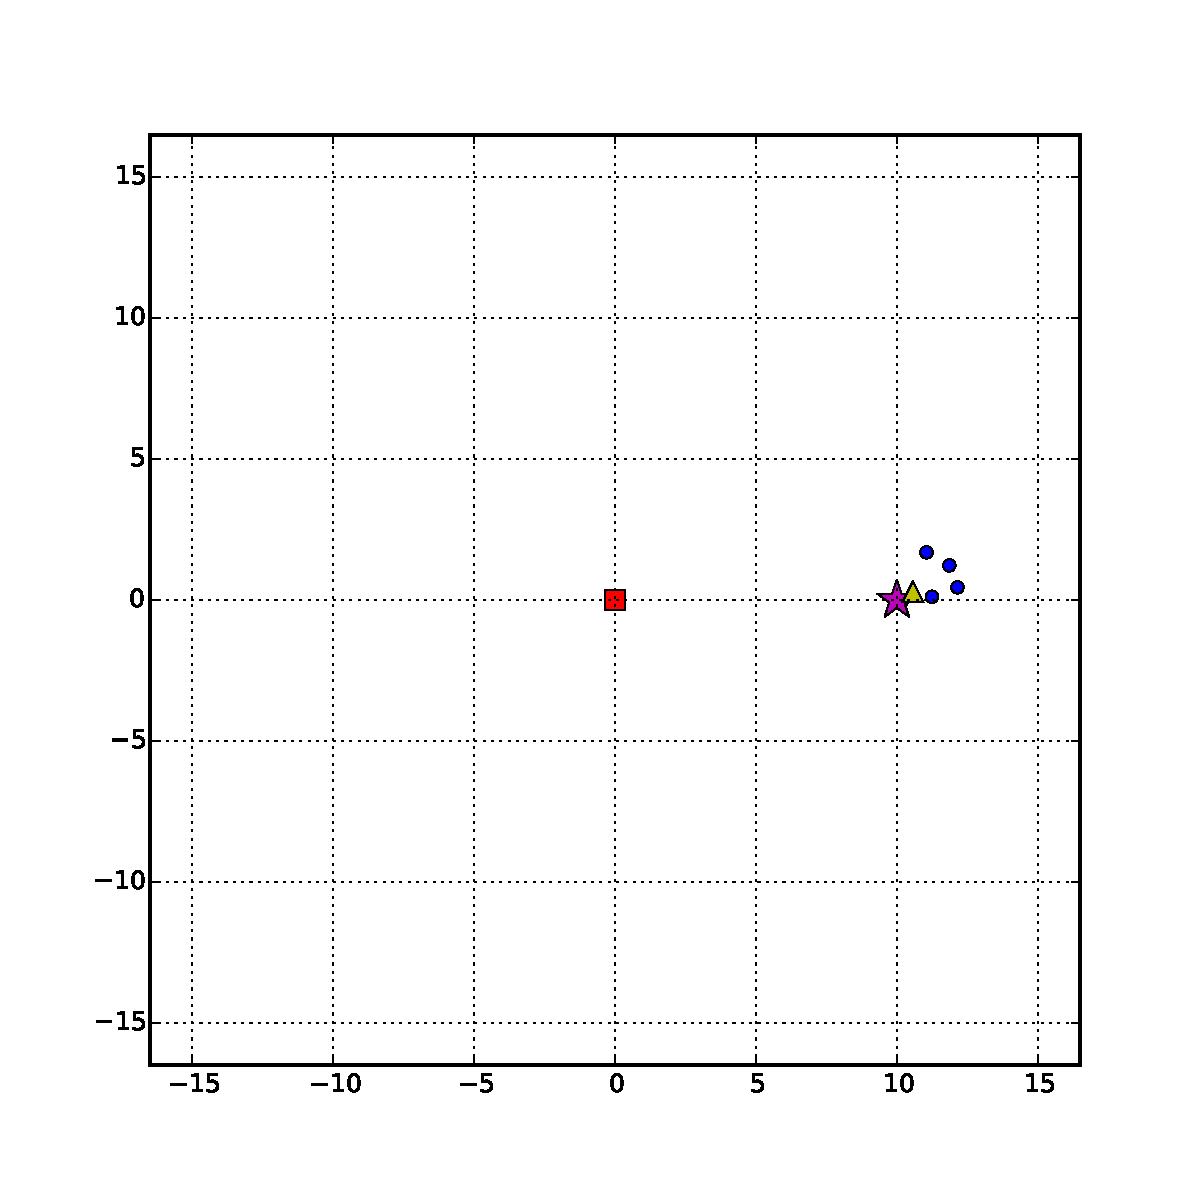
\includegraphics[width=\textwidth]{high_vel_noise_first_obs}
	            \caption{A t=0, first observation}
	            \label{fig:high_vel_noise_t_0}
	    \end{subfigure}
	    ~ %add desired spacing between images, e. g. ~, \quad, \qquad, \hfill etc.
	      %(or a blank line to force the subfigure onto a new line)
	    \begin{subfigure}[b]{0.3\textwidth}
	            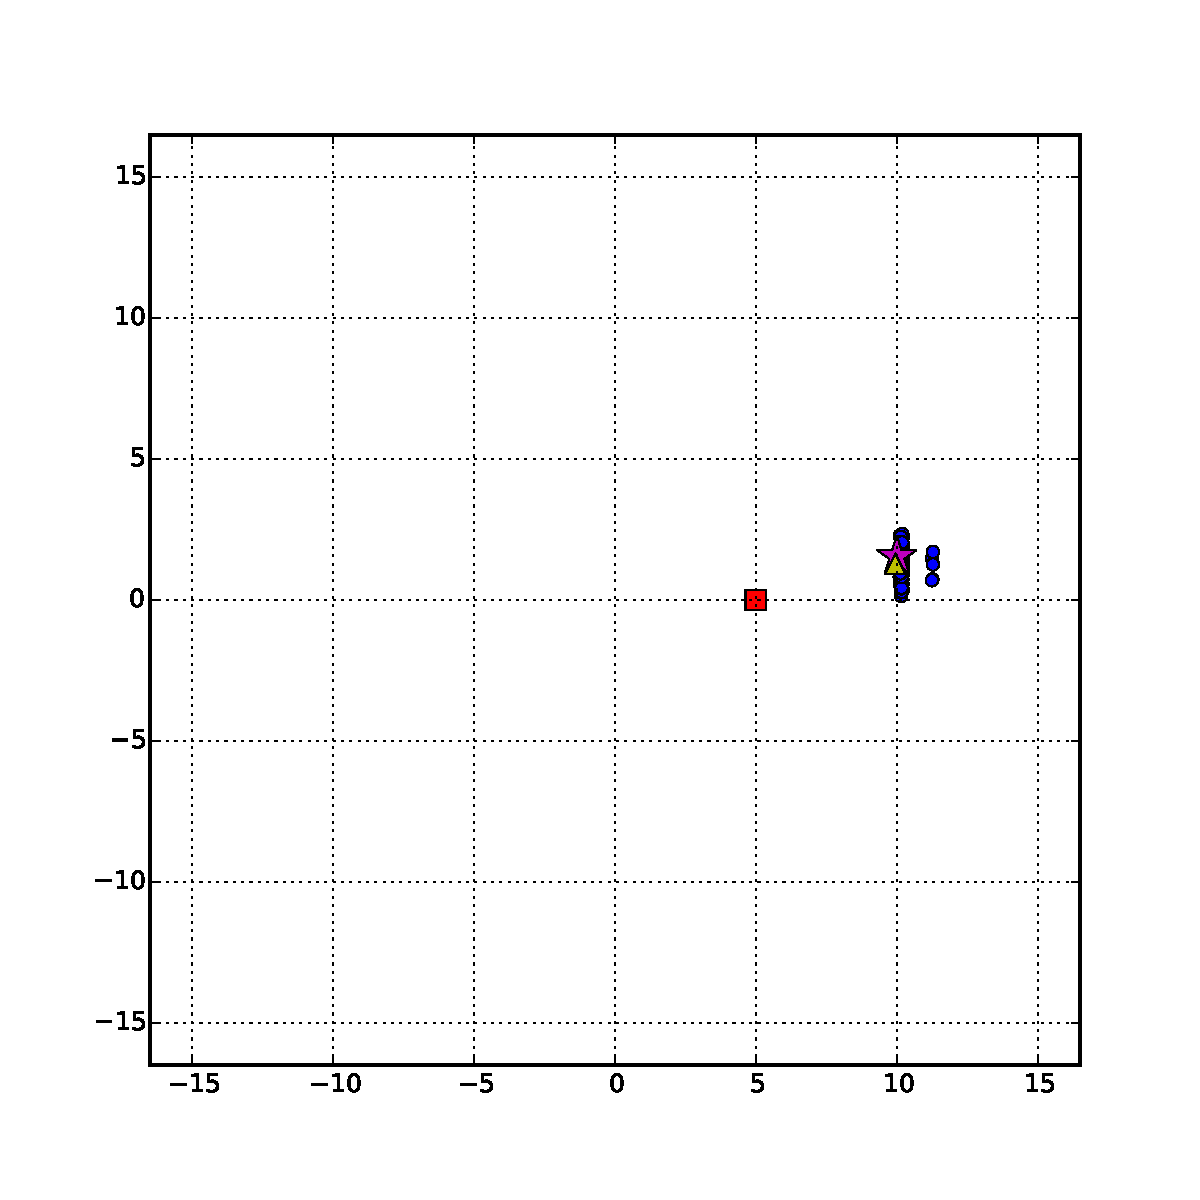
\includegraphics[width=\textwidth]{high_vel_noise_t_1}
	            \caption{t=1}
	            \label{fig:high_vel_noise_t_1}
	    \end{subfigure}
	    \begin{subfigure}[b]{0.3\textwidth}
	            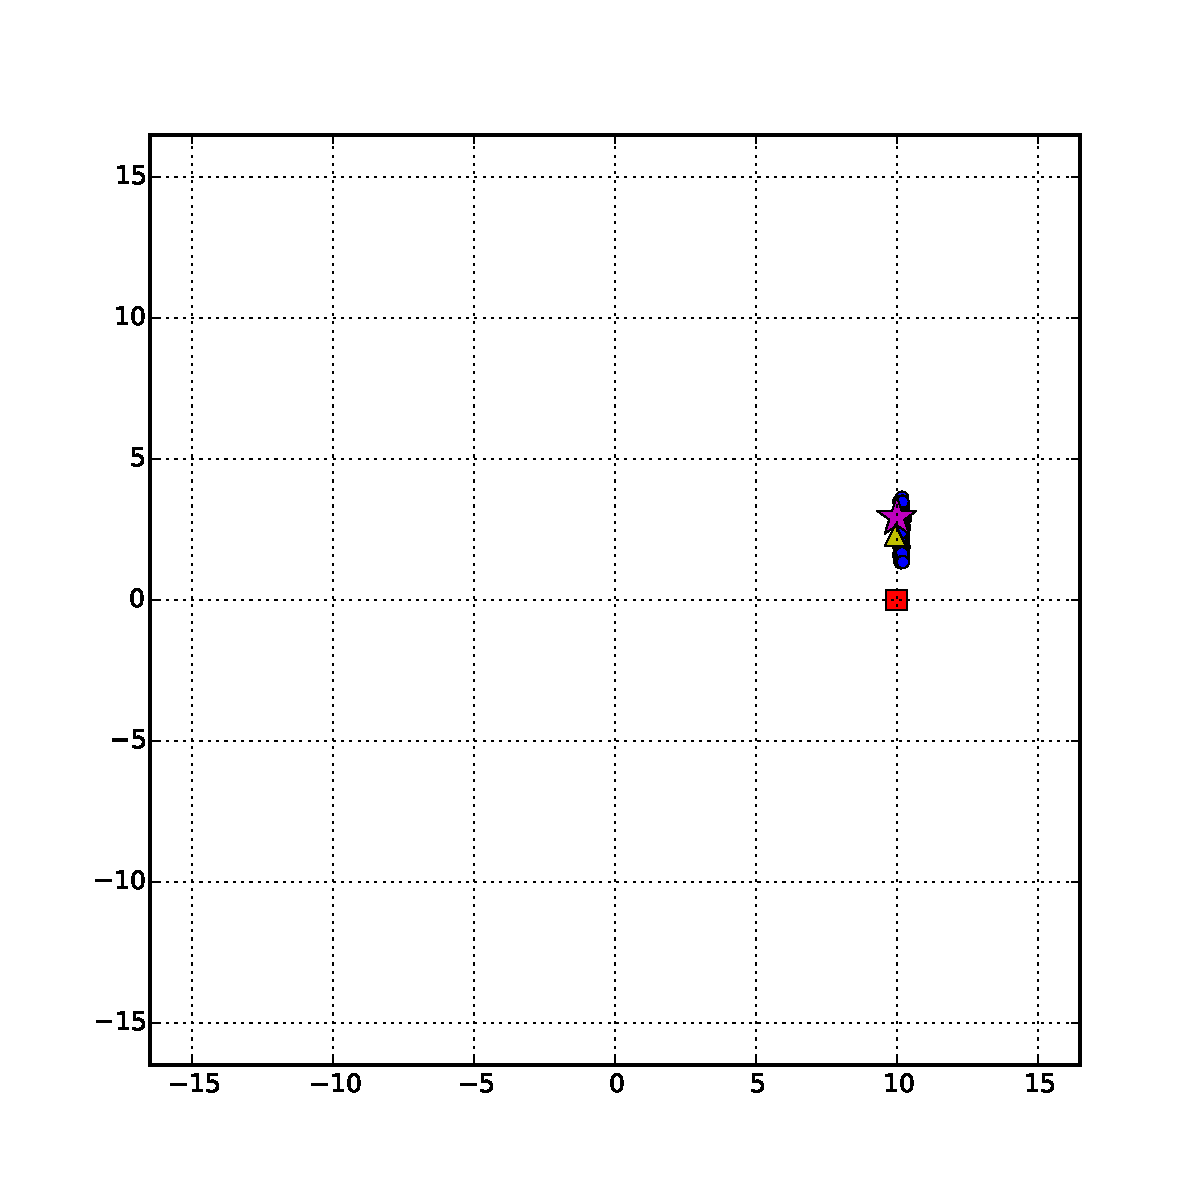
\includegraphics[width=\textwidth]{high_vel_noise_t_2}
	            \caption{t=2}
	            \label{fig:high_vel_noise_t_2}
	    \end{subfigure}
	    \begin{subfigure}[b]{0.3\textwidth}
	            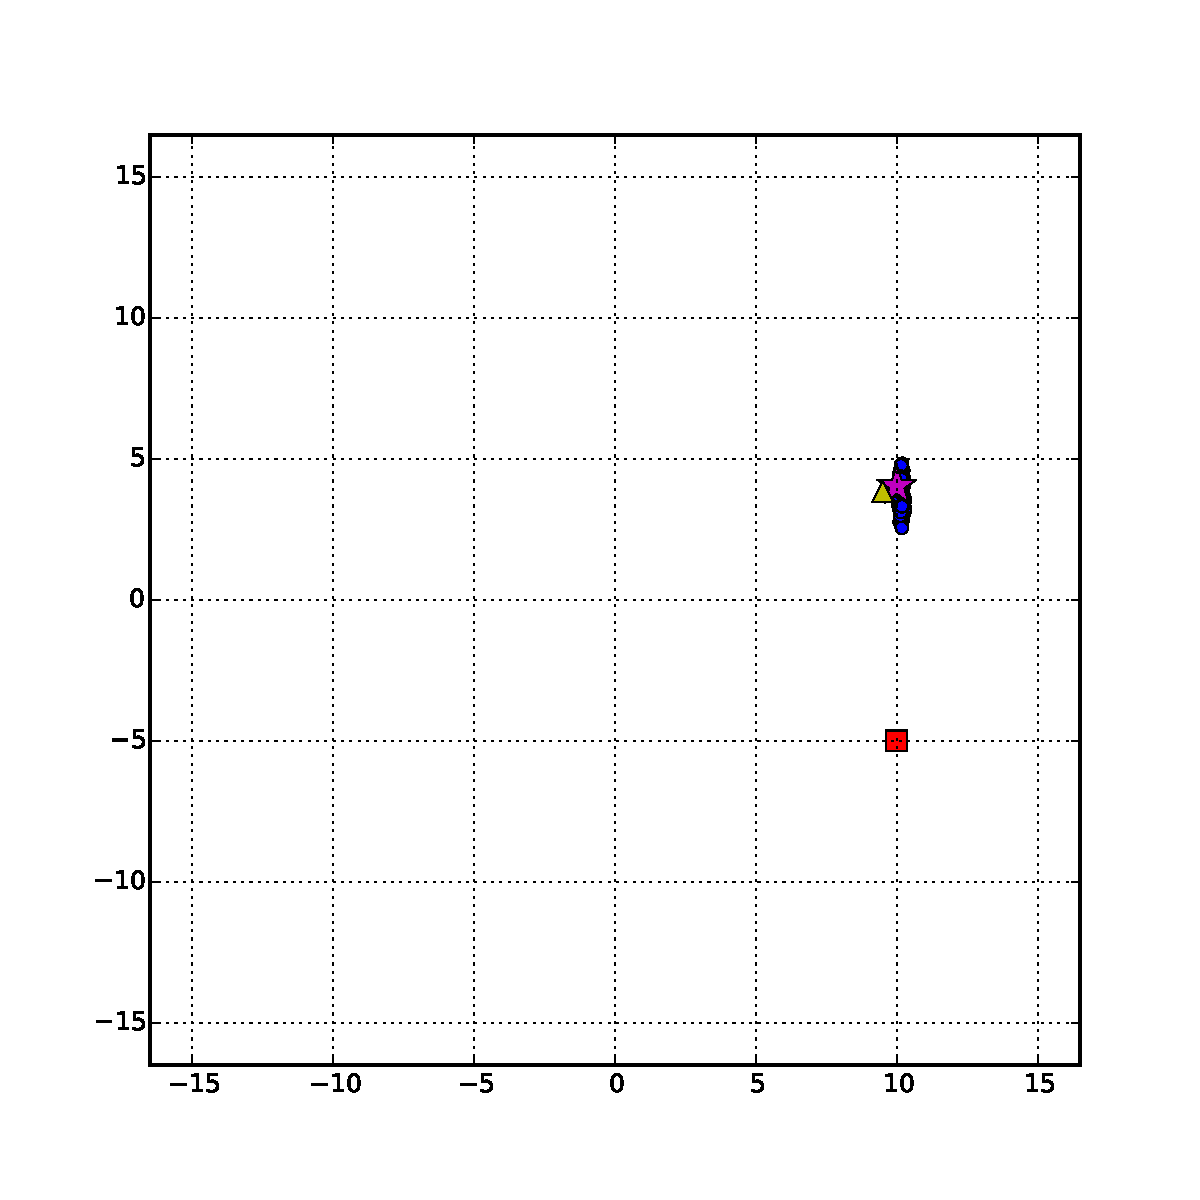
\includegraphics[width=\textwidth]{high_vel_noise_t_3}
	            \caption{t=3}
	            \label{fig:high_vel_noise_t_3}
	    \end{subfigure}
	    \begin{subfigure}[b]{0.3\textwidth}
	            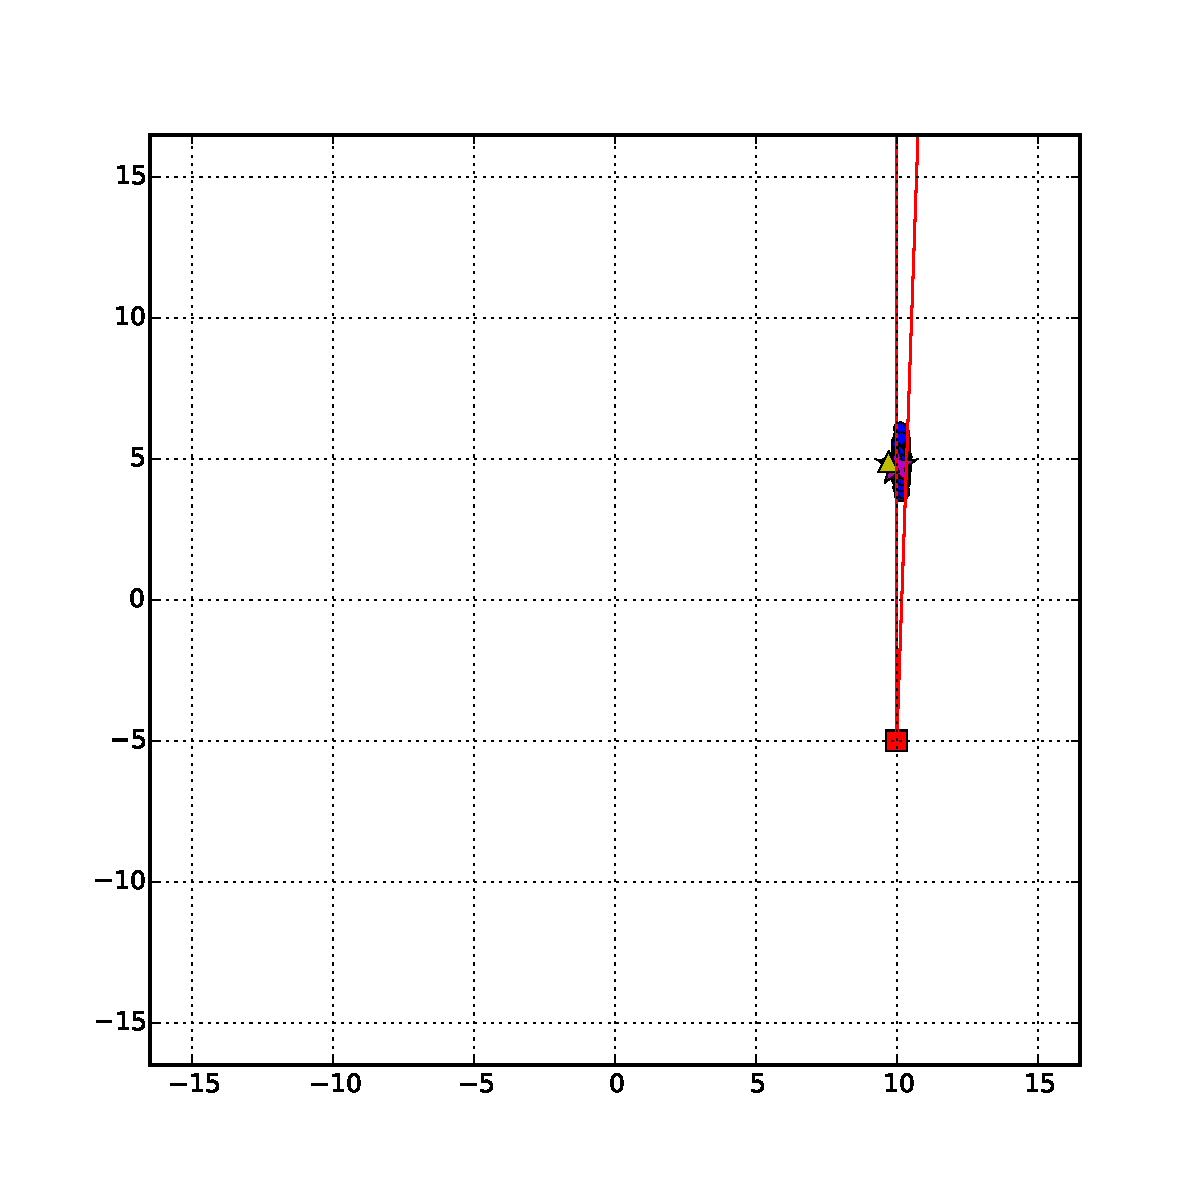
\includegraphics[width=\textwidth]{high_vel_noise_t_4}
	            \caption{t=4, agent egages target}
	            \label{fig:high_vel_noise_t_4}
	    \end{subfigure}
	    \caption{Progression of MC-RTBSS algorithm for the case where there is high velocity noise in the state transition function of the hostile vehicle, and the shooting mechanism is an angle target. The agent state is the red square, the current observation is the yellow triangle, the true target position is the magenta star, the belief state particles are the blue circles, and the shooting mechanism is the red beam.}\label{fig:vel_noise}
	\end{figure}
\break
\subsection{Fixed Improved Vantage Point Model: Point Target}
	In this model we had assumed that there is a fixed location that gives the smallest variance in the observation model, and that the variance increases as the agent is farther away from that location.  The case presented has the improved vantage point at $(-5,10)$.  The visualization of the results can be seen in Figure \ref{fig:vantage}.  In this case the MC-RTBSS algorithm chooses to move toward the vantage point because the uncertainty of the target's location can only be reduced in this way.  The algorithm has computed that the time cost taken to move towards the vantage point will result in a higher score at the end of the game.  This is the behavior that one would expect from an agent behaving rationally in this situation.  As soon as the cost of waiting or moving to improve localization cannot be offset by the expected reward of hitting the target within depth $D$ time steps, the algorithm shoots.  In this example the agent has succeeded in hitting the true target.

	% !TEX root = ./final_report.tex

	\begin{figure}
	        \centering
	        \begin{subfigure}[b]{0.3\textwidth}
	                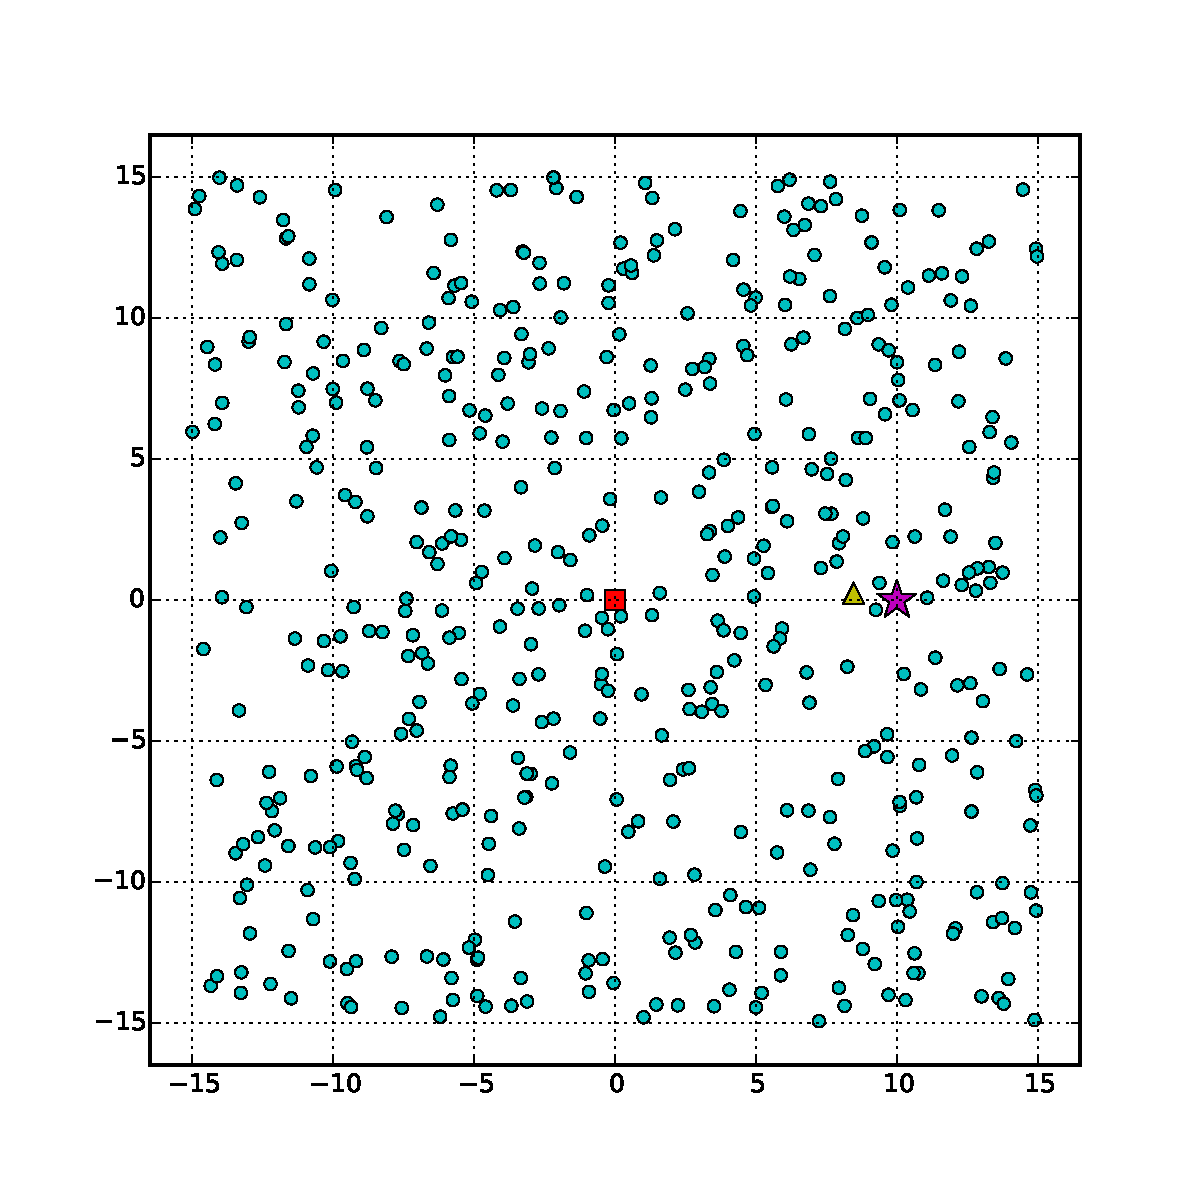
\includegraphics[width=\textwidth]{vantage_initial}
	                \caption{Initial belief state}
	                \label{fig:vantage_init}
	        \end{subfigure}%
	        ~ %add desired spacing between images, e. g. ~, \quad, \qquad, \hfill etc.
	          %(or a blank line to force the subfigure onto a new line)
	        \begin{subfigure}[b]{0.3\textwidth}
	                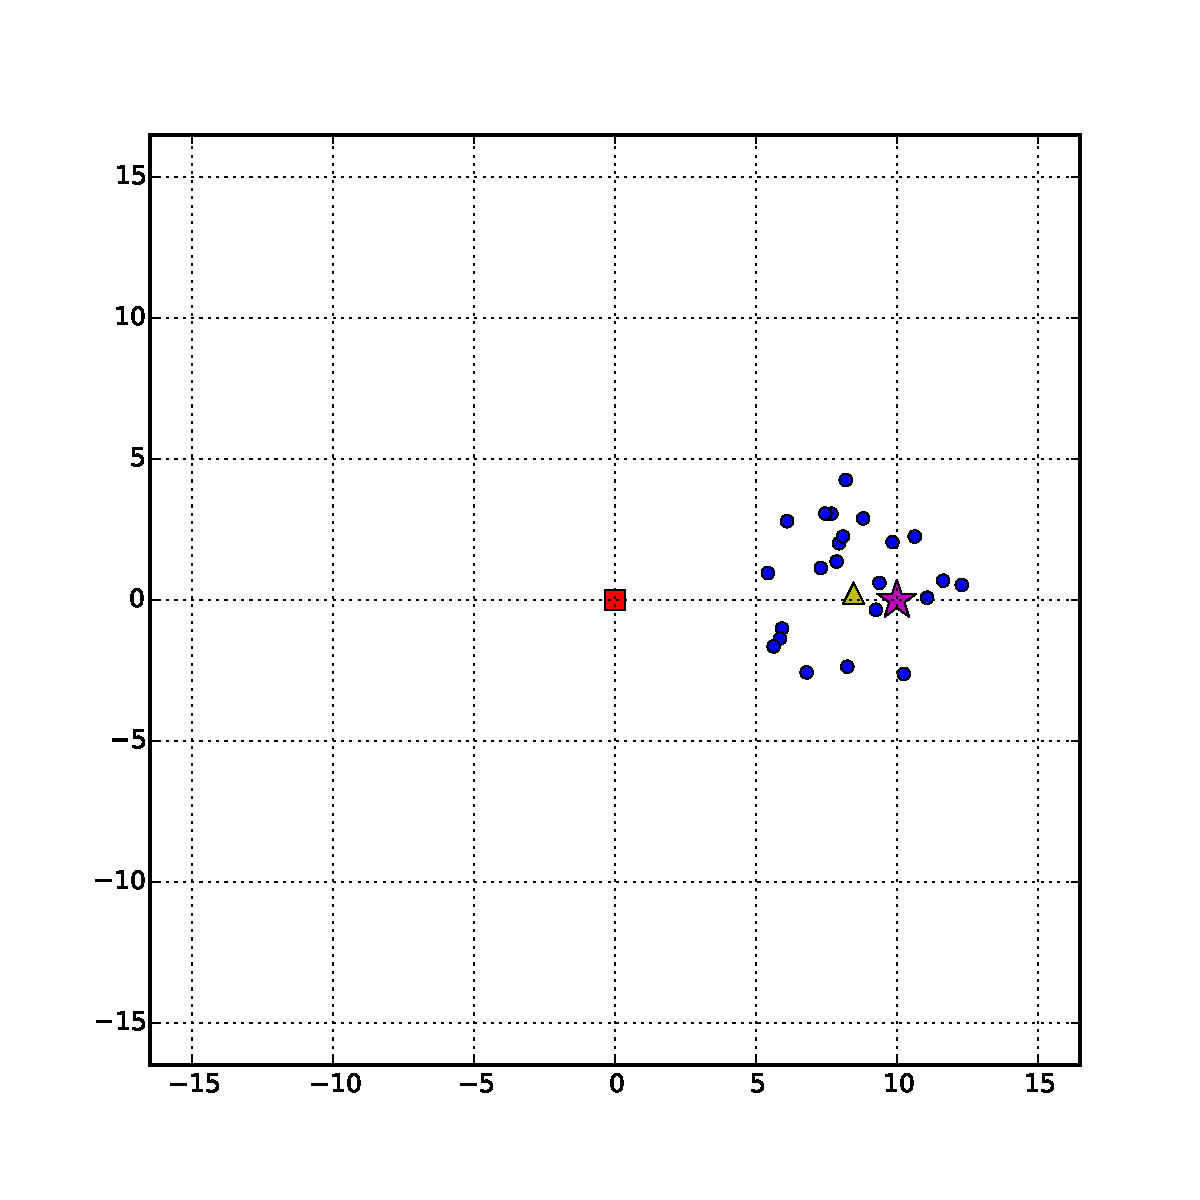
\includegraphics[width=\textwidth]{vantage_first_obs}
	                \caption{A t=0, first observation}
	                \label{fig:vantage_t_0}
	        \end{subfigure}
	        ~ %add desired spacing between images, e. g. ~, \quad, \qquad, \hfill etc.
	          %(or a blank line to force the subfigure onto a new line)
	        \begin{subfigure}[b]{0.3\textwidth}
	                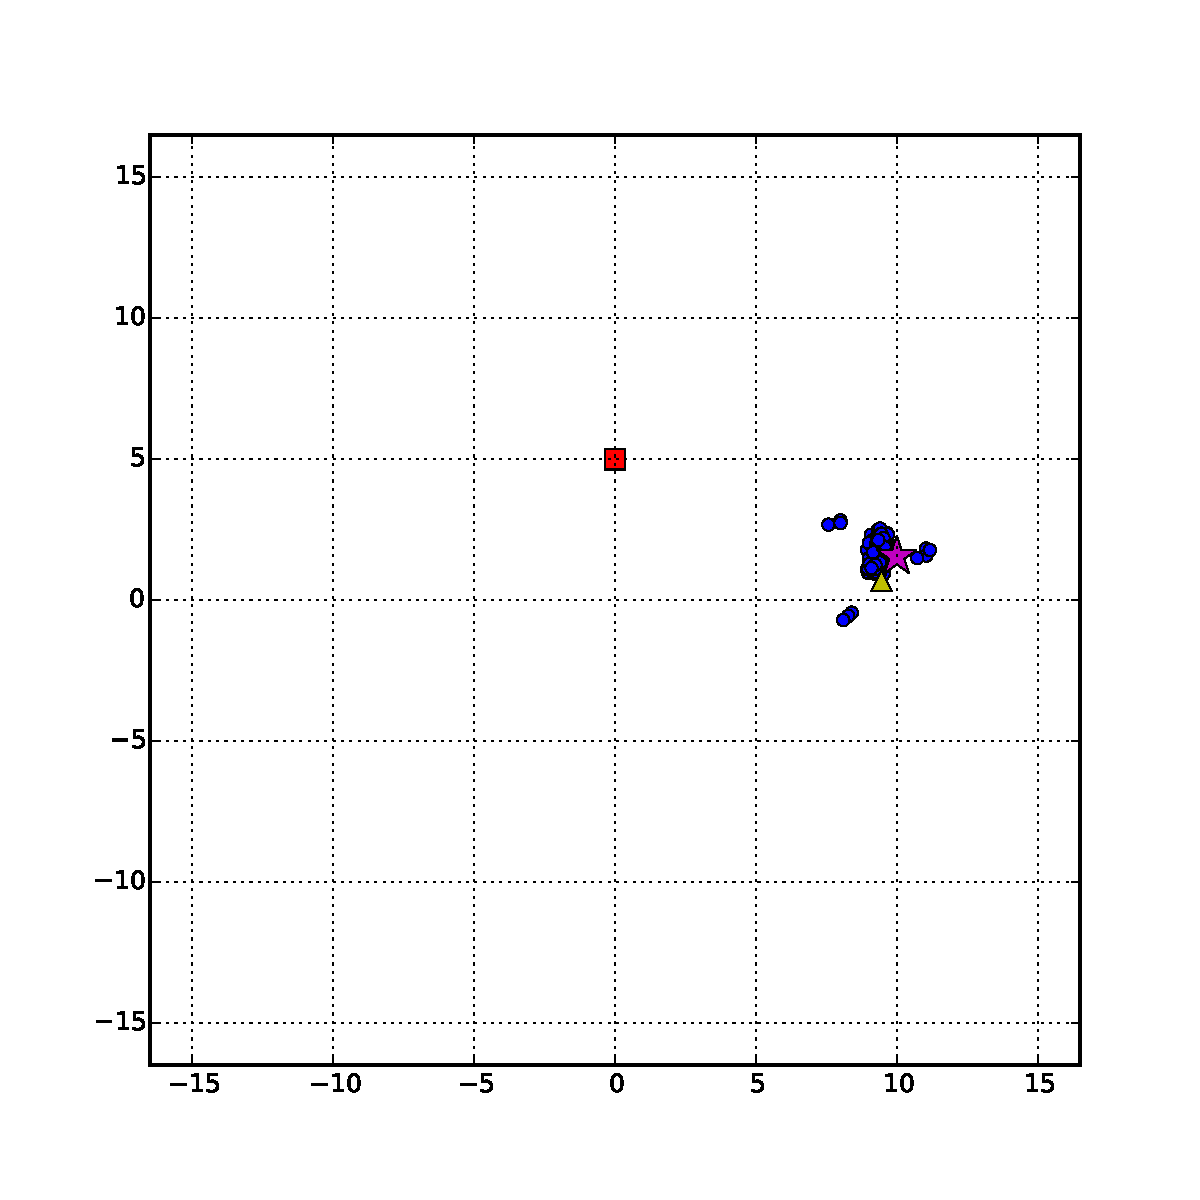
\includegraphics[width=\textwidth]{vantage_t_1}
	                \caption{t=1}
	                \label{fig:vantage_t_1}
	        \end{subfigure}
	        \begin{subfigure}[b]{0.3\textwidth}
	                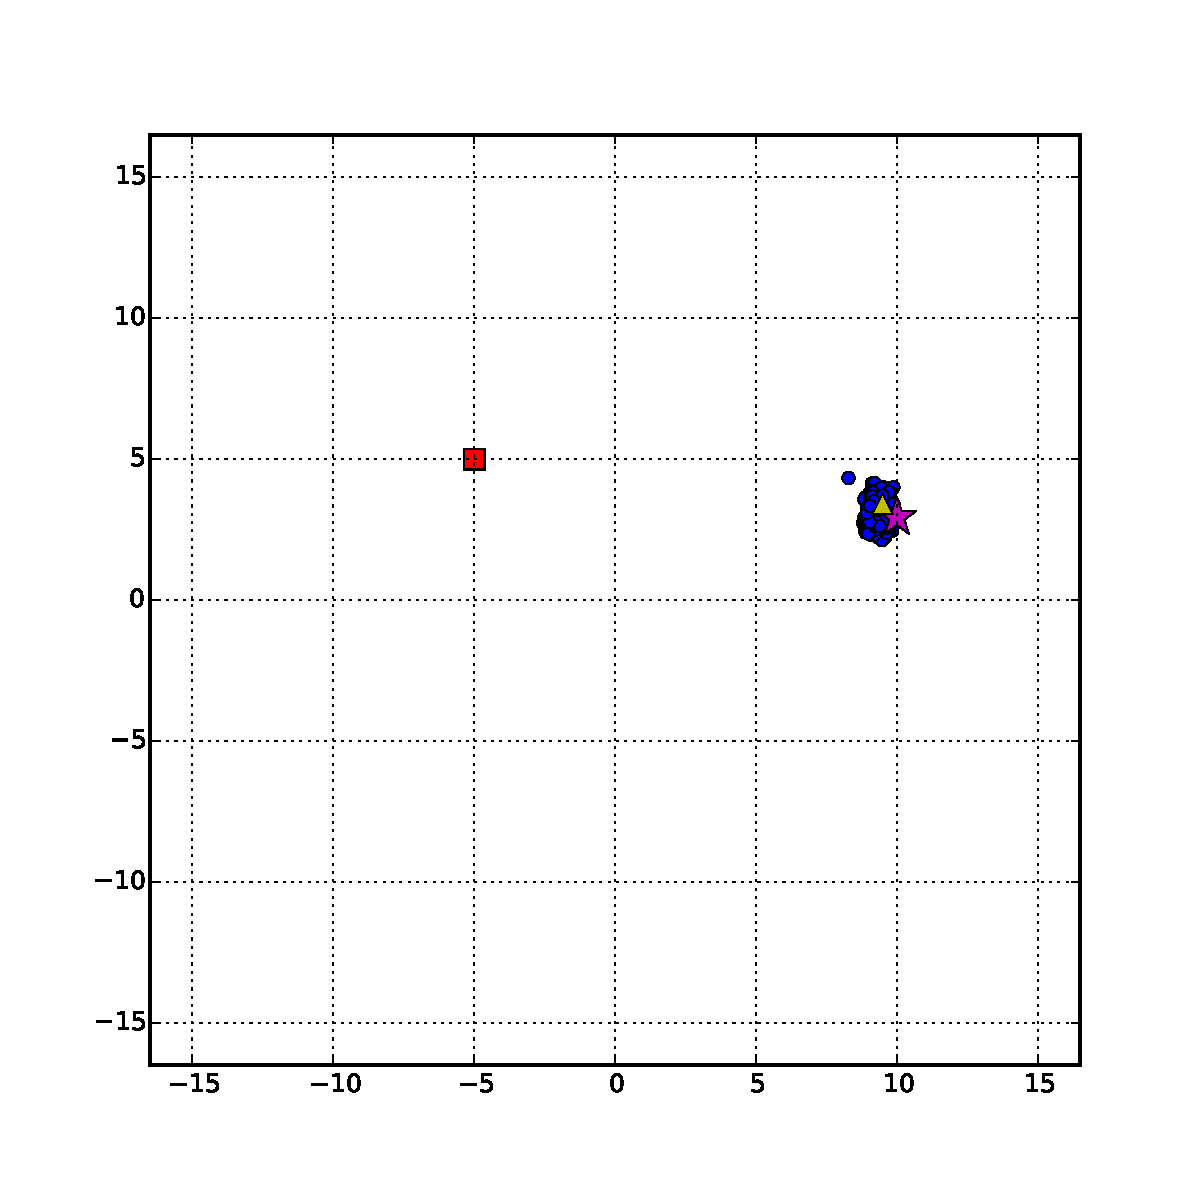
\includegraphics[width=\textwidth]{vantage_t_2}
	                \caption{t=2}
	                \label{fig:vantage_t_2}
	        \end{subfigure}
	        \begin{subfigure}[b]{0.3\textwidth}
	                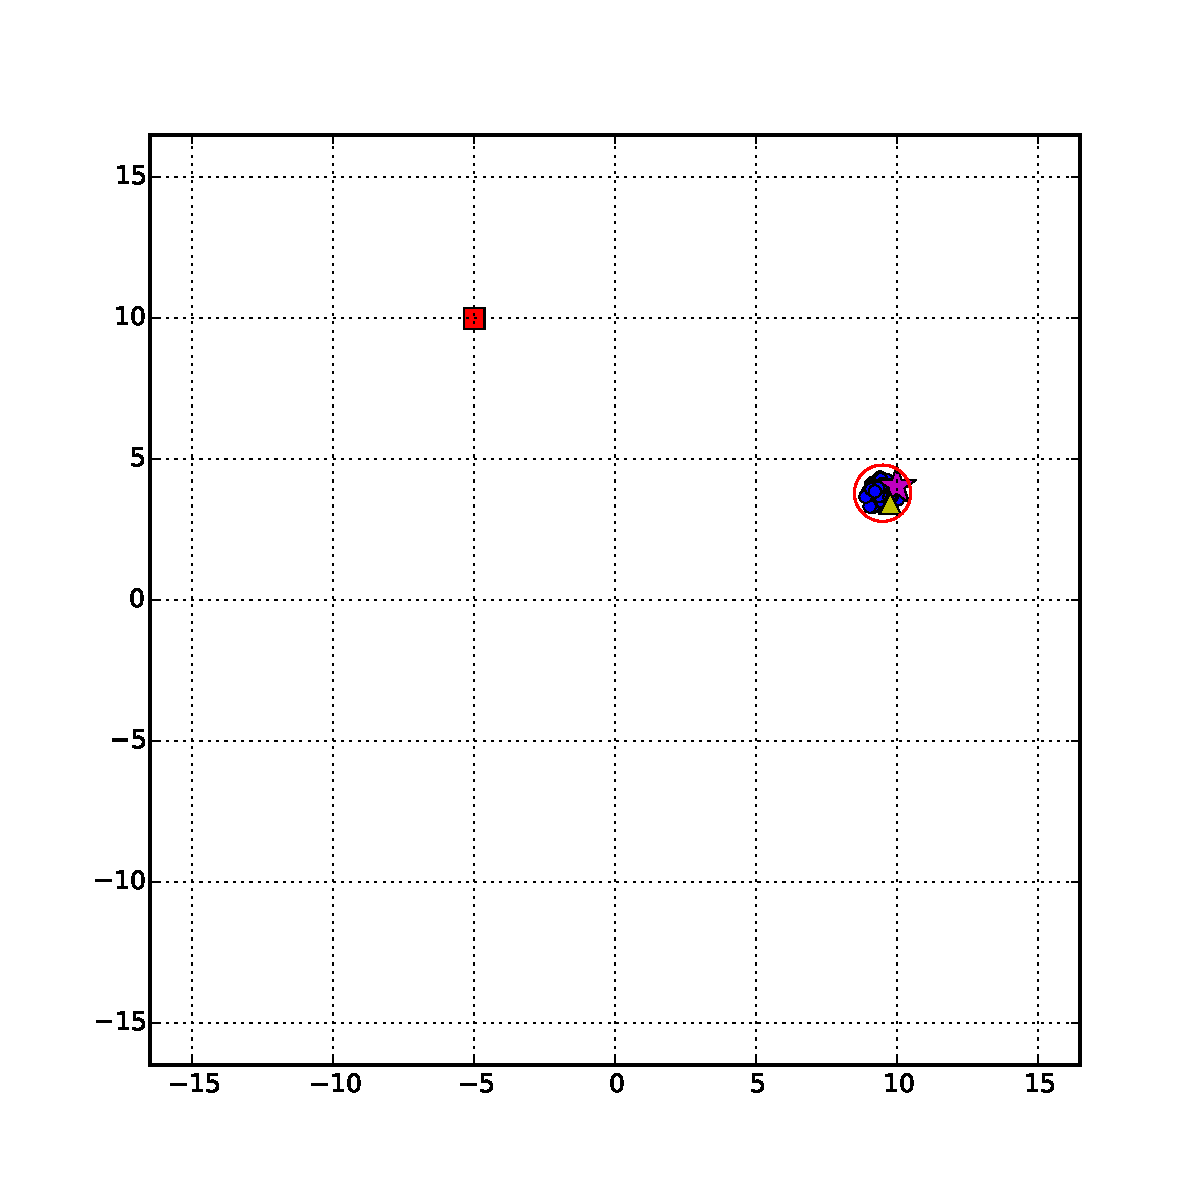
\includegraphics[width=\textwidth]{vantage_t_3}
	                \caption{t=3, agent engages target}
	                \label{fig:vantage_t_3}
	        \end{subfigure}
	        \caption{Progression of MC-RTBSS algorithm for the case where an improved vantage point exists at $(-5,10)$, and the shooting mechanism is a point target. The agent state is the red square, the current observation is the yellow triangle, the true target position is the magenta star, the belief state particles are the blue circles, and the shooting mechanism is the red circle.}\label{fig:vantage}
	\end{figure}
	